%%%%%%%%%%%%%%%%%%%%%%%%%%%%%%%%%%%%%%%%%%%%%%%%%%%%%%%%%%%%%%%%%%%%%%%%%%%%%%%%
%
% https://www.sharelatex.com/learn/Beamer
%
%%%%%%%%%% 
\documentclass{beamer}
	\usetheme{ACUAS}
%	\usetheme{Madrid}
%
% 	- Hiding the presentation controls in LaTeX beamer presentation [closed]
%		- https://stackoverflow.com/questions/3017030/hiding-the-presentation-controls-in-latex-beamer-presentation
%	\usetheme{Dresden}
%		\usecolortheme{beaver}
	\setbeamertemplate{navigation symbols}{}
	%
	% Gitterllinien auf den Folien anzeigen
	%
	%\beamertemplategridbackground[1cm]


%%%%%%%%%%%%%%%%%%%%%%%%%%%%%%%%%%%%%%%%%%%%%%%%%%%%%%%%%%%%%%%%%%%%%%%%%%%%%%%%
%
% Packages
%
%%%%%%%%%% 
\usepackage{fontspec}
\usepackage{lmodern}
\usepackage{polyglossia}
	\setmainlanguage[variant=german, spelling=new]{german}
\usepackage{graphicx}
	\graphicspath{{./logos/}{./bilder/}}

%
% bibtex vs. biber and biblatex vs. natbib
%	- https://tex.stackexchange.com/questions/25701/bibtex-vs-biber-and-biblatex-vs-natbib
% The biblatex Package - Programmable Bibliographies and Citations
% 	- http://ftp.math.purdue.edu/mirrors/ctan.org/macros/latex/exptl/biblatex/doc/biblatex.pdf
% Biblatex citation order
%	- https://tex.stackexchange.com/questions/51434/biblatex-citation-order
% 		- sorting=ydnt: Sort by year (descending), name, title.
%		- sorting=none: Do not sort at all. All entries are processed in citation order.
%
\usepackage[
	backend=biber,
	style=numeric-comp,
	%style=ieee,
	sorting=none,
]{biblatex}
	\addbibresource{quellen.bib}
	
%\usepackage{showframe}

\usepackage[mode=text]{siunitx}
	\sisetup{locale=DE, range-phrase=--, product-units=single, binary-units=true}
	\DeclareSIUnit{\mAh}{mAh}
	\DeclareSIUnit{\belmilliwatt}{Bm}
	\DeclareSIUnit{\dBm}{\deci\belmilliwatt}
	
\usepackage{subcaption}

	% How to remove figure caption prefix “figure” in beamer
	% https://tex.stackexchange.com/questions/82456/how-to-remove-figure-caption-prefix-figure-in-beamer
	\captionsetup[figure]{labelformat=empty}


%%%%%%%%%%%%%%%%%%%%%%%%%%%%%%%%%%%%%%%%%%%%%%%%%%%%%%%%%%%%%%%%%%%%%%%%%%%%%%%%
%
% Information to be included in the title page
%
%%%%%%%%%%
\title[RO-SLAM mittels UWB]{Range-Only Simultaneous Localization and Mapping mittels Ultra-Wideband}
%\subtitle{}
\author[A. Kasdorf]
{
	Albert Kasdorf\\
	Matr.-Nr.: 3029294
}
\institute[FH Aachen]
{
	FH Aachen\\
	Fachbereich Elektrotechnik und Informationstechnik\\
	Ingenieur-Informatik
}
\date{26.02.2018}


\begin{document}


%%%%%%%%%%%%%%%%%%%%%%%%%%%%%%%%%%%%%%%%%%%%%%%%%%%%%%%%%%%%%%%%%%%%%%%%%%%%%%%%
%
% Titelseite
%
%%%%%%%%%%
\frame{\titlepage}


%%%%%%%%%%%%%%%%%%%%%%%%%%%%%%%%%%%%%%%%%%%%%%%%%%%%%%%%%%%%%%%%%%%%%%%%%%%%%%%%
%
% Inhaltsverzeichnis?
%
%%%%%%%%%%
%\begin{frame}
%\frametitle{Inhaltsverzeichnis}
%\tableofcontents
%\end{frame}


%%%%%%%%%%%%%%%%%%%%%%%%%%%%%%%%%%%%%%%%%%%%%%%%%%%%%%%%%%%%%%%%%%%%%%%%%%%%%%%%
%
% 
%
%%%%%%%%%%
\part{Einführung}


%%%%%%%%%%%%%%%%%%%%%%%%%%%%%%%%%%%%%%%%%%%%%%%%%%%%%%%%%%%%%%%%%%%%%%%%%%%%%%%%
%
%	- Was ist das Ziel? (Karte mit Beacons und Roboterpose)
%		- Was ist Lokalisierung?
%		- Was ist Kartenerstellung?
%	- Was ist SLAM?
%	- Was ist RO-SLAM?
%	- Wie kommt man da hin?
%	- Welche Informationen stehen bereit? ((Laserbasierte und Inkrementalgeberbasierte)Odometrie und Entfernungsmessungen)
%	- Findet eine Triangulation statt? (Nein, die ist auch nicht notwendig.)
%		- Trilateration und Multilateration
%		- Lateration
%		- https://de.wikipedia.org/wiki/Lateration#Trilateration_und_Multilateration
%
%%%%%%%%%%
\begin{frame}{Einführung - Lokalisierung, Kartenerstellung, SLAM, RO-SLAM}
	\begin{columns}
		\begin{column}{0.5\linewidth}
			\begin{overlayarea}{\textwidth}{.35\textheight}
				\only<1>
				{
					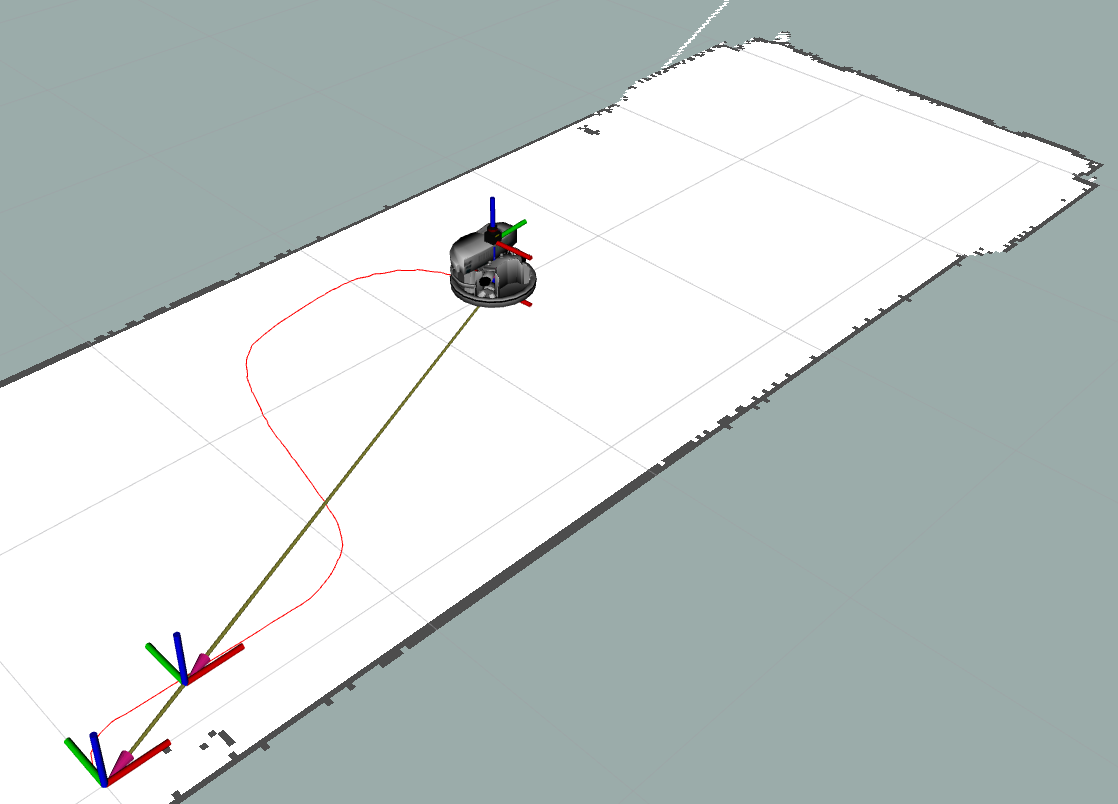
\includegraphics[width=\linewidth]{intro_localization}
				}
				\only<2>
				{
					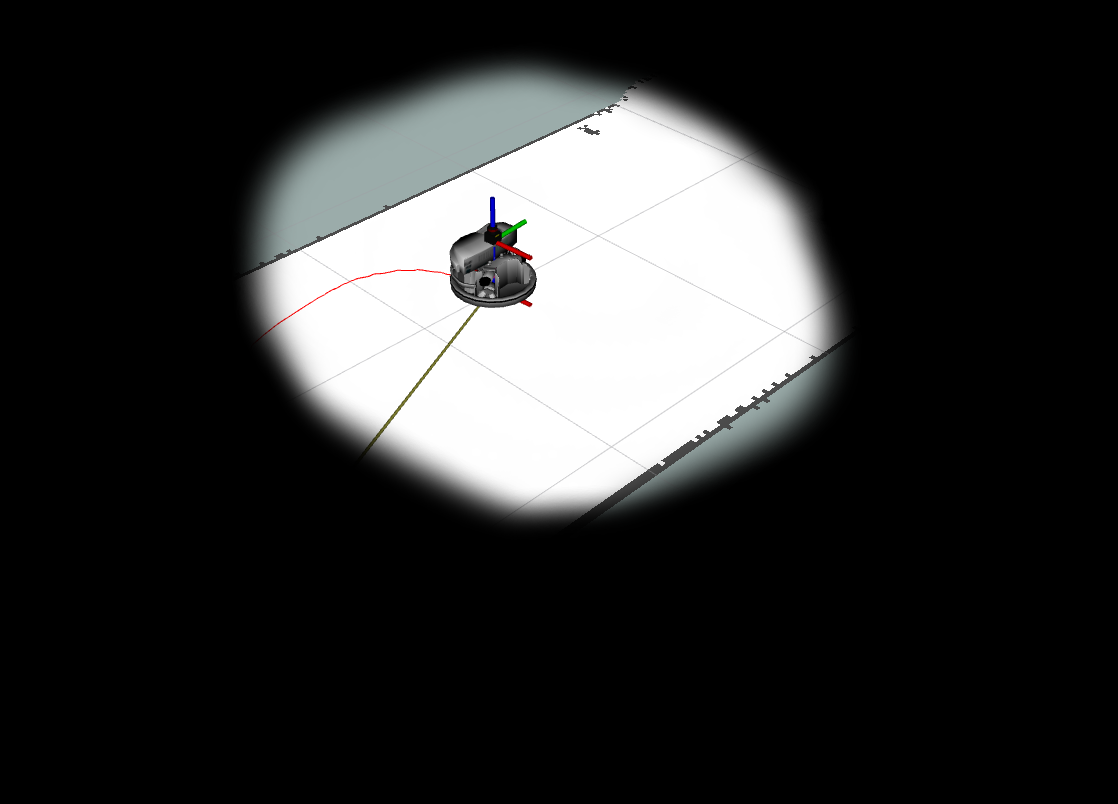
\includegraphics[width=\linewidth]{intro_mapping}
				}
				\only<3>
				{
					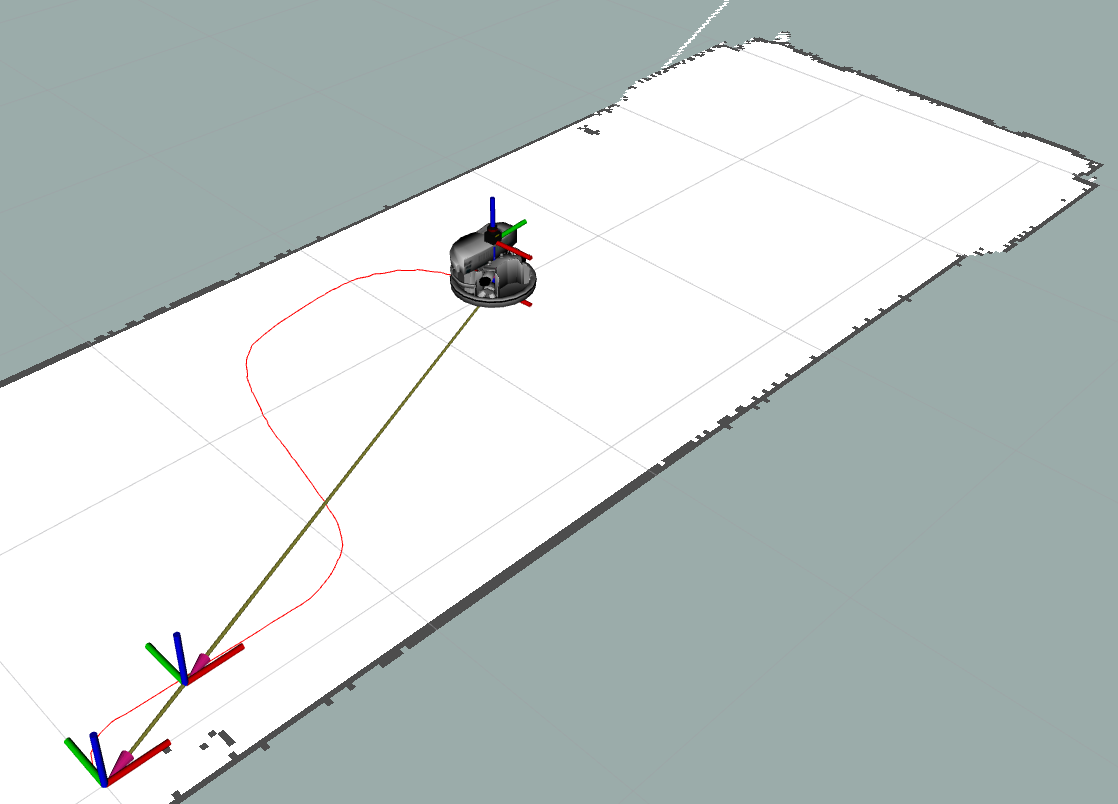
\includegraphics[width=\linewidth]{intro_localization}
				}
				\only<4>
				{
					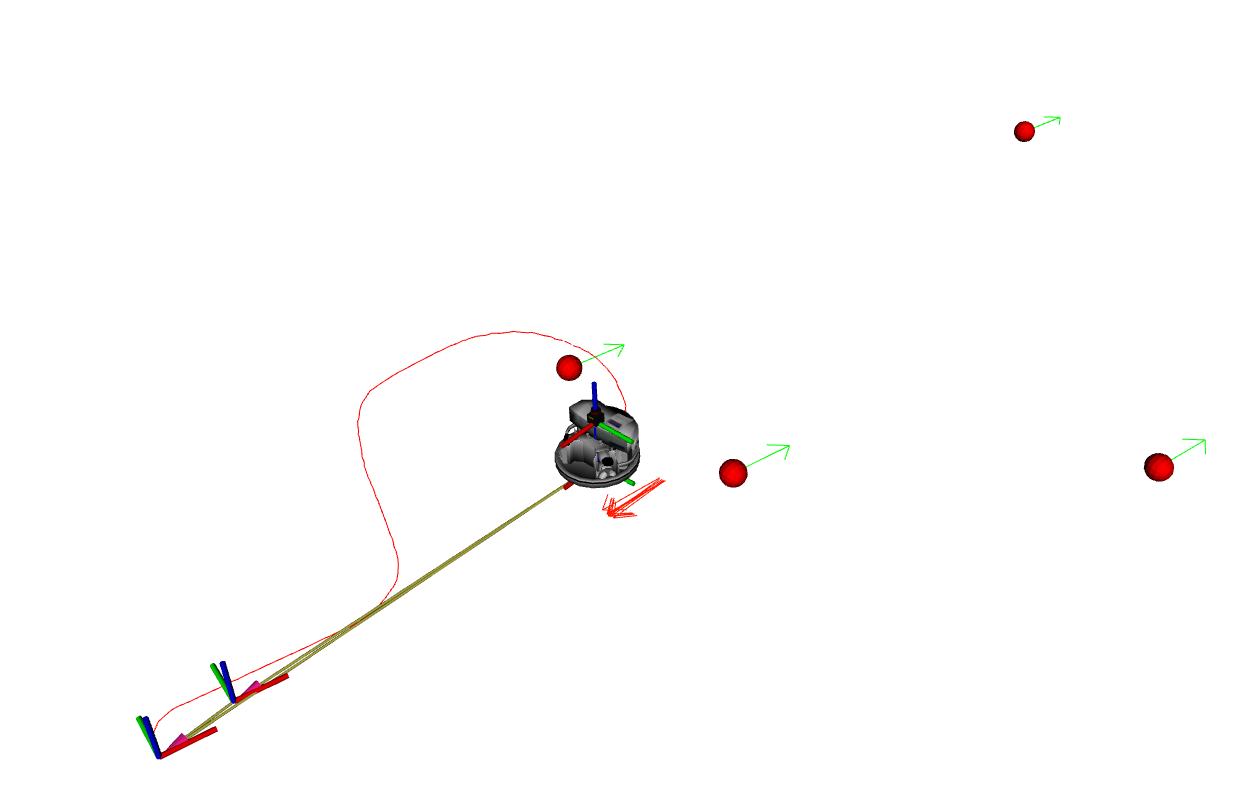
\includegraphics[width=\linewidth]{intro_roslam1}
				}
				\only<5>
				{
					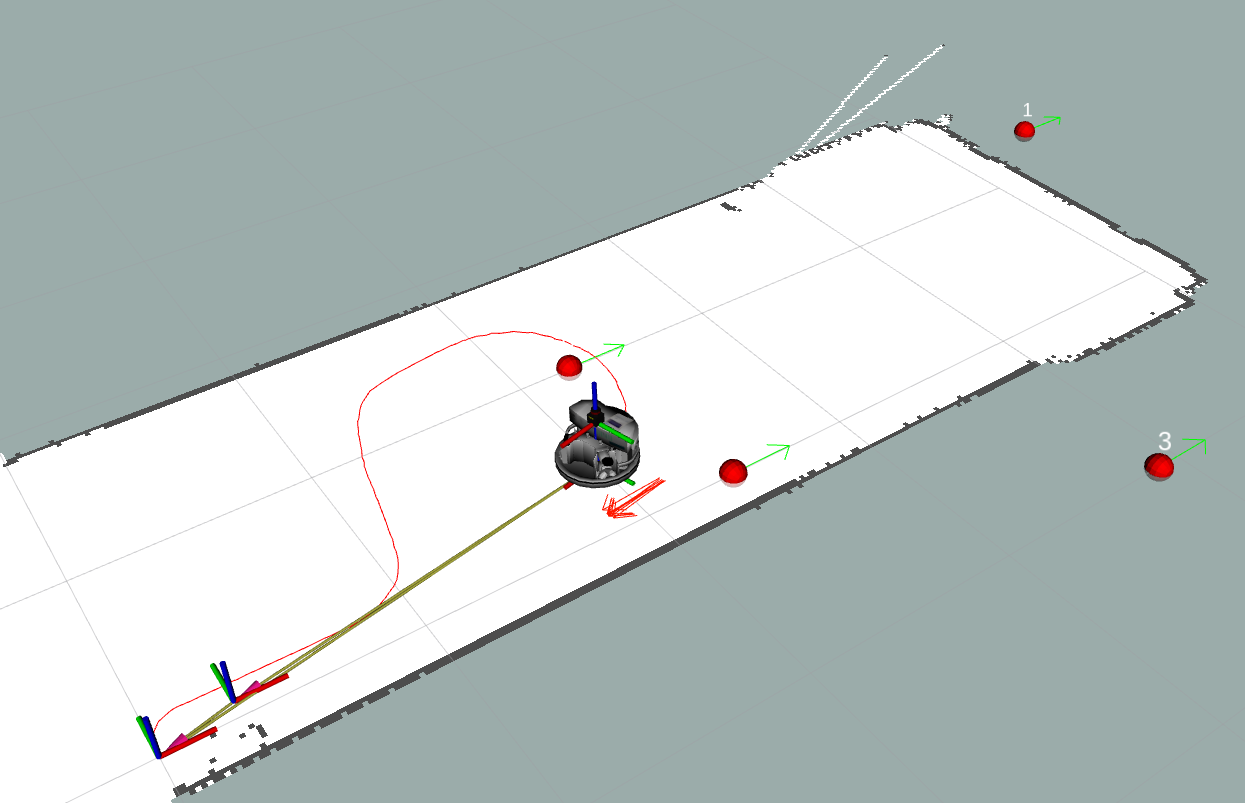
\includegraphics[width=\linewidth]{intro_roslam2}
				}
			\end{overlayarea}
		\end{column}
		%\hspace{-50pt} 
		%\vrule{}
		\begin{column}{0.5\linewidth}
			\begin{itemize}
				\item<1-> Lokalisierung
				\item<2-> Kartenerstellung
				\item<3-> SLAM
				\item<4-> RO-SLAM
			\end{itemize}
		\end{column}
	\end{columns}
\end{frame}


%%%%%%%%%%%%%%%%%%%%%%%%%%%%%%%%%%%%%%%%%%%%%%%%%%%%%%%%%%%%%%%%%%%%%%%%%%%%%%%%
%
% 
%
%%%%%%%%%%
\part{Ultra-Wideband}


%%%%%%%%%%%%%%%%%%%%%%%%%%%%%%%%%%%%%%%%%%%%%%%%%%%%%%%%%%%%%%%%%%%%%%%%%%%%%%%%
%
%	- Was ist UWB?
%		- Was sind die wichtigsten Eigenschaften für den RO-SLAM?
%	- Aus welchen Komponenten besteht das Modul?
%		- UWB Tranciever von DecaWave
%	- todo
%		- Neues Bild aufnehmen
%	- Unterschied zwischen Landmarke, Beacon, Anker, Tag, UWB Modul?
%		- Landmarke: Ausgezeichnetes Merkmal der Umwelt
%		- Beacon/Leuchtfeuer/Funkbarke: Landmarke auf Funkbasis
%		- Anker: Beacon der als Referenzpunkt dient und sich nicht bewegt
%		- Tag: Beacon der sich bewegen kann
%		- UWB Modul: Konkrete technische Umsetzung eines Beacons
%
%%%%%%%%%%
\begin{frame}{UWB Modul - Erstellte Hardware}
	\begin{columns}
		\begin{column}{0.5\linewidth}
			\centering
			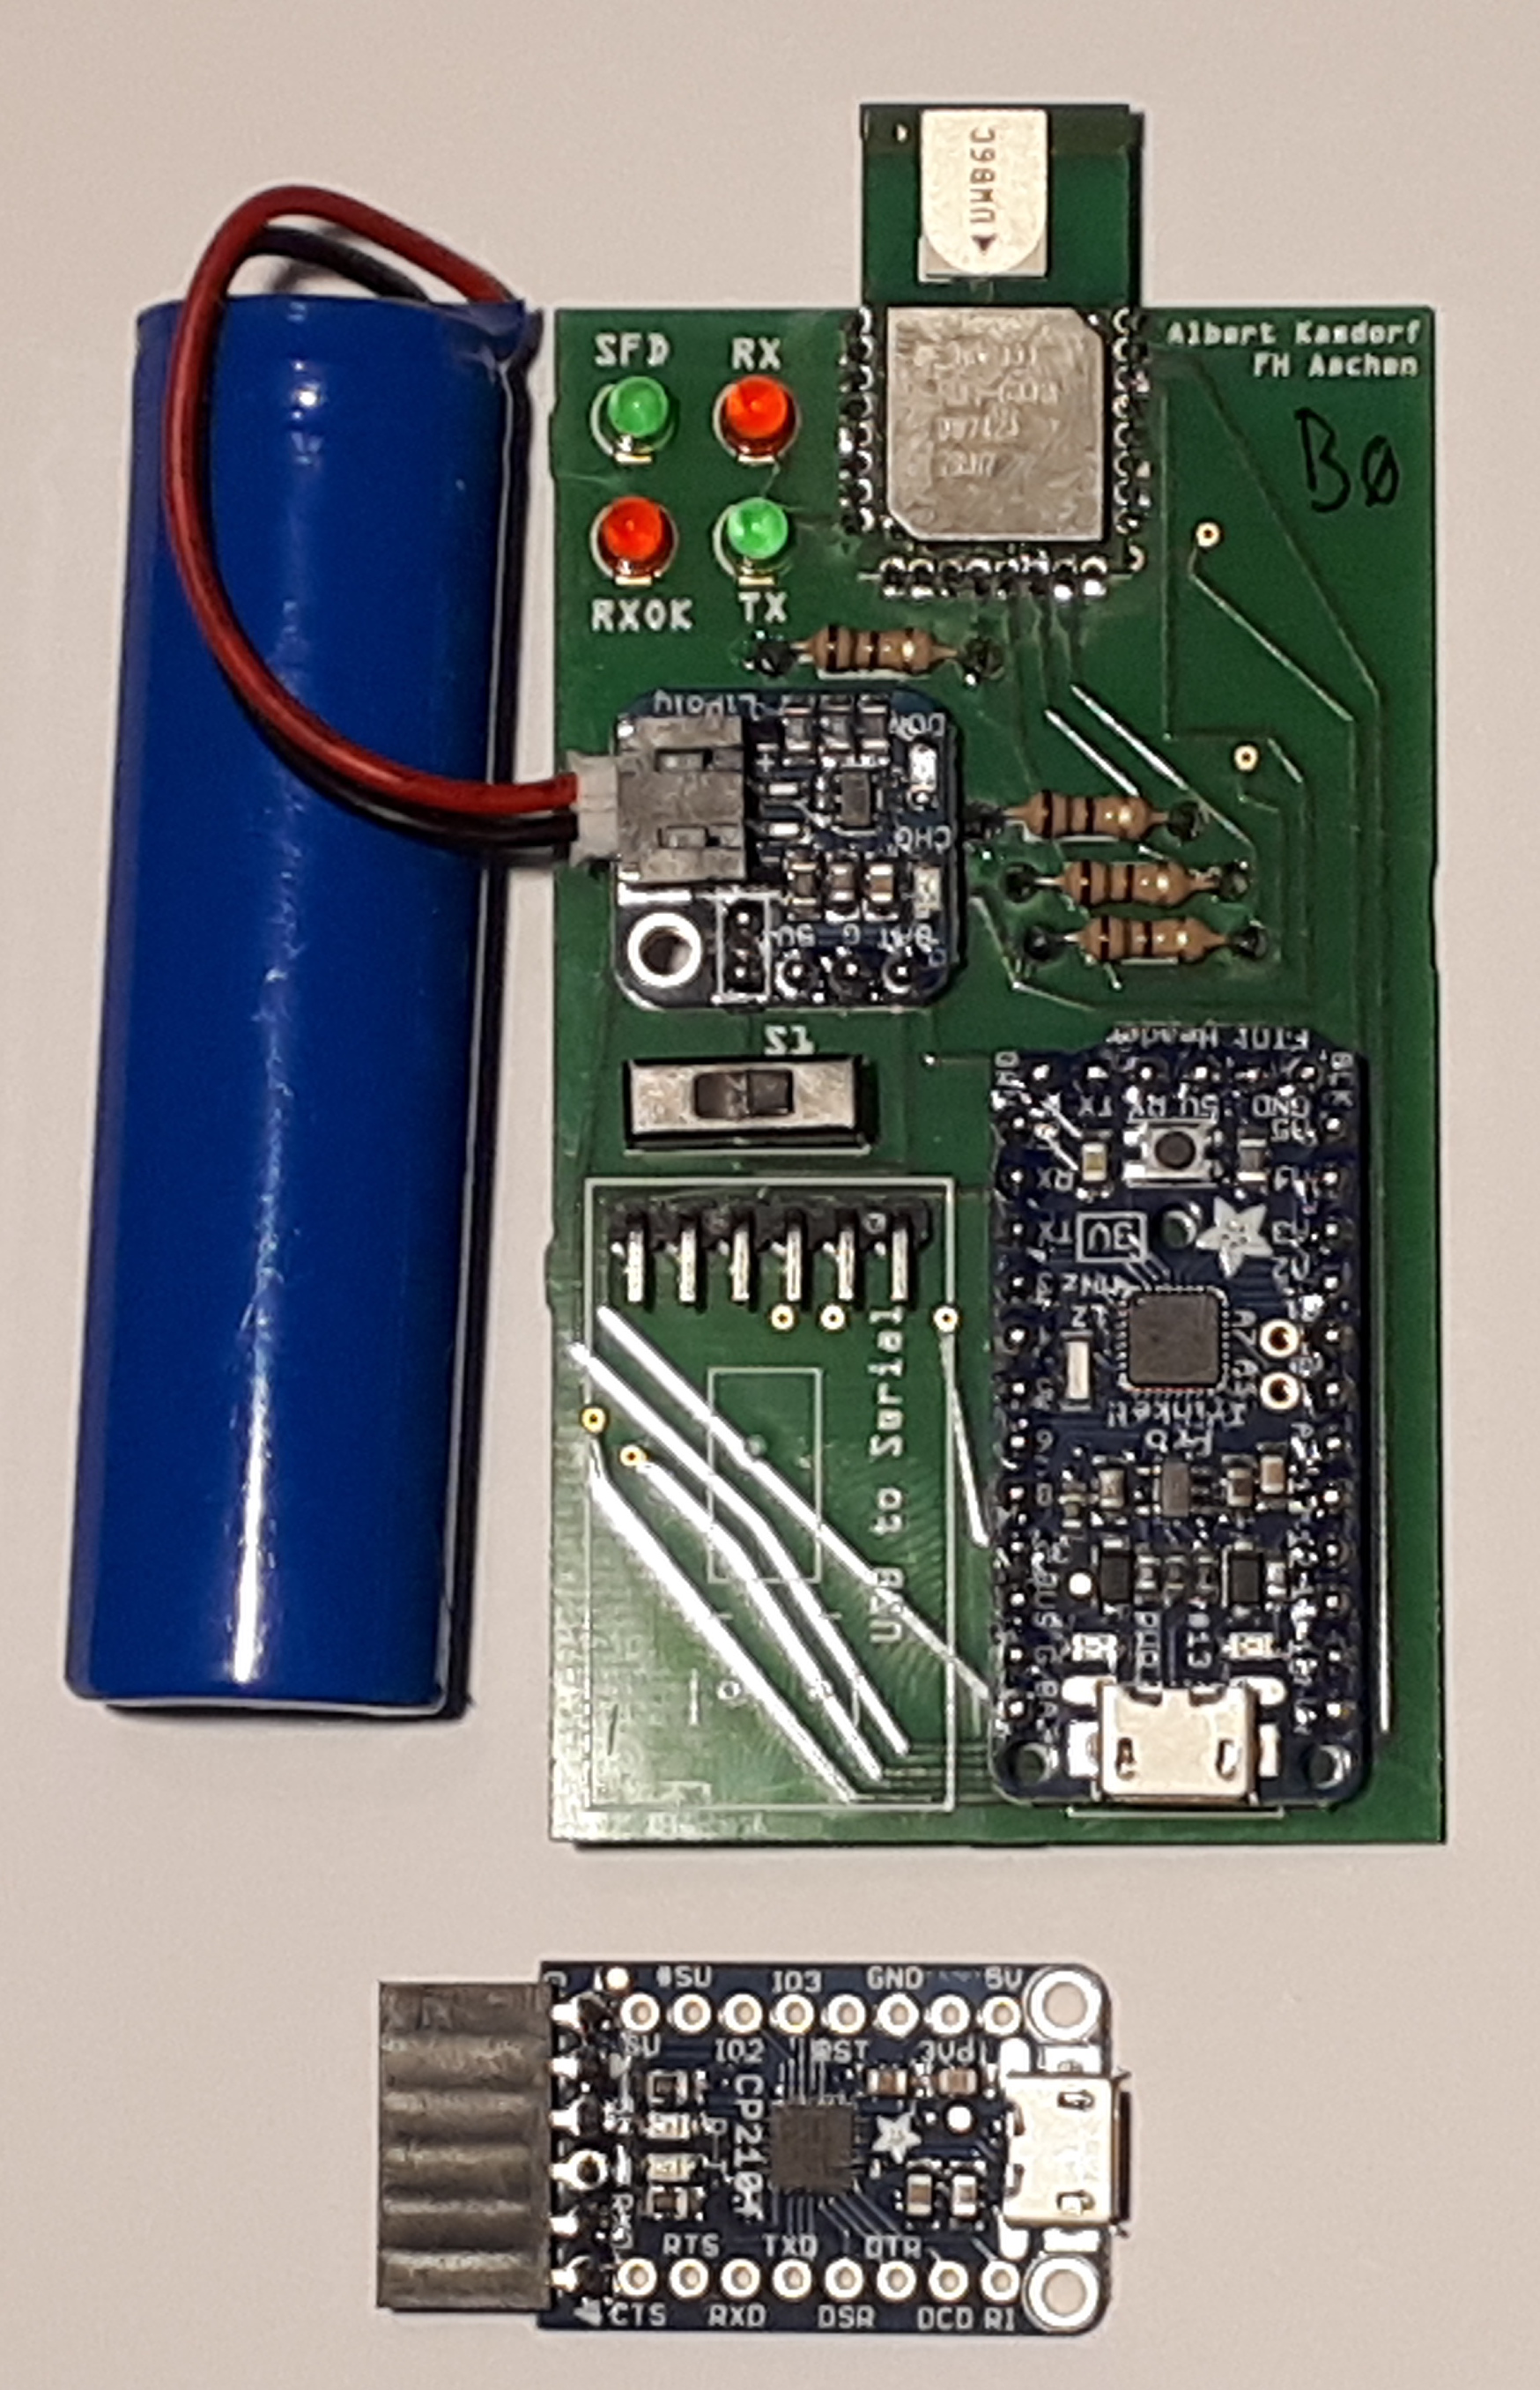
\includegraphics[width=0.8\linewidth]{uwb_modul2}
		\end{column}
		\begin{column}{0.5\linewidth}
			\begin{itemize}
				\item<1-> UWB
				\begin{itemize}
					\item Basisband, keine Modulation
					\item Bandbreite bis zu \SI{500}{\MHz}
				\end{itemize}
				\item<2-> Begrifflichkeiten
				\begin{itemize}
					\item Landmarke, Beacon
					\item Anker, Tag, UWB Modul
				\end{itemize}
				\item<3-> UWB Modul
				\begin{itemize}
					\item DecaWave Transceiver
					\item Hardwareplattform
					\item Energieversorgung
				\end{itemize}
			\end{itemize}
		\end{column}
	\end{columns}
\end{frame}


%%%%%%%%%%%%%%%%%%%%%%%%%%%%%%%%%%%%%%%%%%%%%%%%%%%%%%%%%%%%%%%%%%%%%%%%%%%%%%%%
%
%	- Warum muss überhaupt kalibiert werden?
%
%%%%%%%%%%
\begin{frame}{Kalibierung (1/3) - Bestimmung der Antennenverzögerung}
	\begin{columns}
		\begin{column}{0.5\linewidth}
			\begin{figure}
				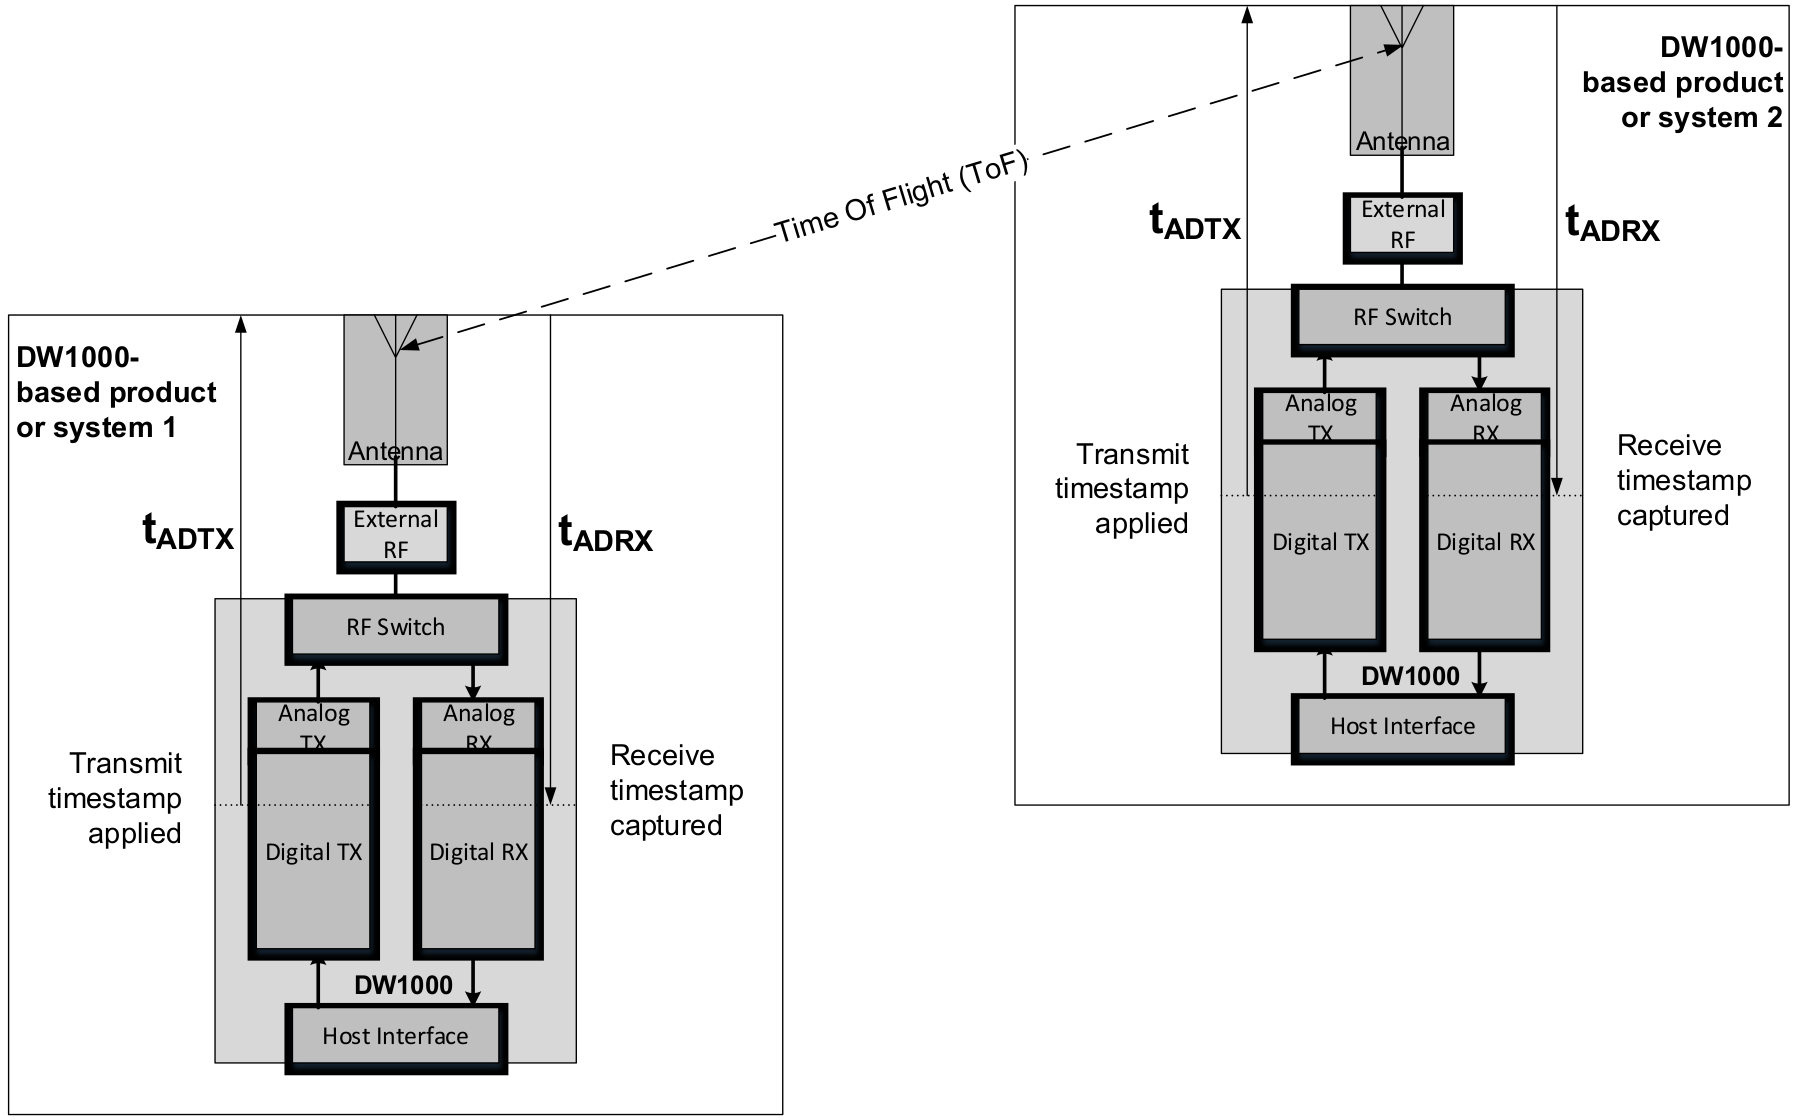
\includegraphics[width=\linewidth]{decawave2014calibration_fig1}
				\caption{\cite{decawave2014calibration}}
			\end{figure}
		\end{column}
		\begin{column}{0.5\linewidth}
			\begin{itemize}
				\item Antennenverzögerung
				\item DecaWave Verfahren
					\begin{itemize}
						\item Genetischer Algorithmus
						\item Instabiles Verfahren
					\end{itemize}
				\item LGS Verfahren
					\begin{itemize}
						\item $t_{ad1} + t_{ad2} = tof_{measured} - tof_{actual}$
					\end{itemize}
			\end{itemize}
		\end{column}
	\end{columns}
\end{frame}


%%%%%%%%%%%%%%%%%%%%%%%%%%%%%%%%%%%%%%%%%%%%%%%%%%%%%%%%%%%%%%%%%%%%%%%%%%%%%%%%
%
%	- Warum wurde ein regelmäßiges Fünfeck / Pentagramm verwendet?
%		- Nur zwei unterschiedliche Längen
%		- Der Radius reicht vollkommen aus um alle anderen Seiten zu berechen
%
%%%%%%%%%%
\begin{frame}{Kalibierung (2/3) - Versuchsaufbau}
	\centering
	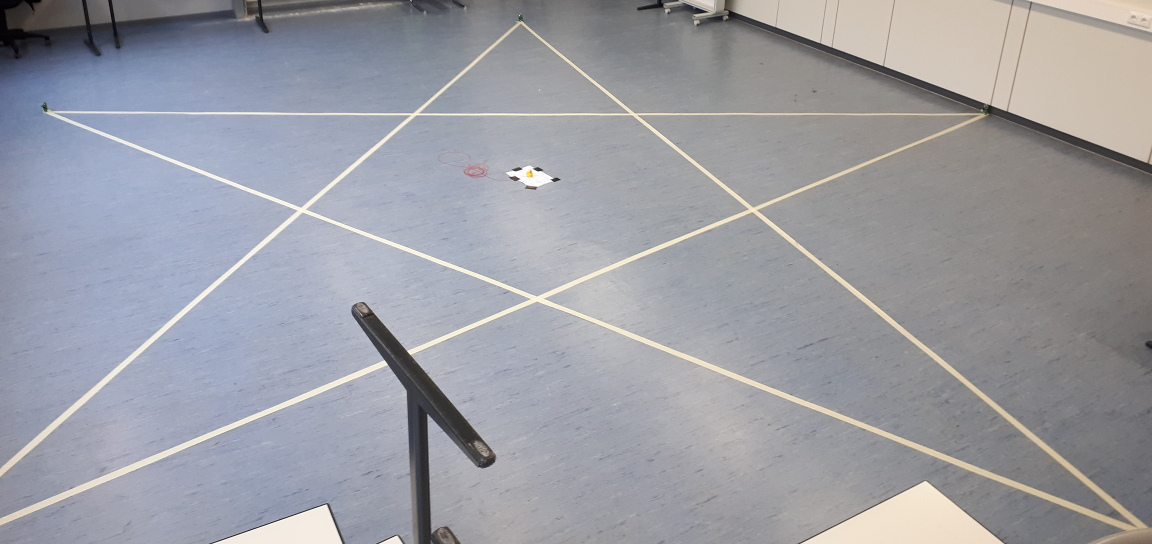
\includegraphics[width=\linewidth]{calibration_pentagram2}
\end{frame}


%%%%%%%%%%%%%%%%%%%%%%%%%%%%%%%%%%%%%%%%%%%%%%%%%%%%%%%%%%%%%%%%%%%%%%%%%%%%%%%%
%
%
%
%%%%%%%%%%
\begin{frame}{Kalibierung (3/3) - Auswertung}
	\begin{table}
		\centering
		\begin{tabular}{||c||c||ccc||}
			\hline
			UWB Modul & LGS & DecaWave & DecaWave 1 & DecaWave 2 \\
			& [\si{\nano\second}] & [\si{\nano\second}] & [\si{\nano\second}] & [\si{\nano\second}] \\
			\hline
			\hline
			176 & \num{257.45} & \num{242.48} & \num{232.21} & \num{254.50} \\
			177 & \num{257.49} & \num{238.47} & \num{249.38} & \num{254.73} \\
			178 & \num{257.11} & \num{257.17} & \num{255.36} & \num{215.07} \\
			\hline
		\end{tabular}
		%\caption{Berechnete Werte für die Antennenverzögerung pro UWB Modul.}
	\end{table}
\end{frame}


%%%%%%%%%%%%%%%%%%%%%%%%%%%%%%%%%%%%%%%%%%%%%%%%%%%%%%%%%%%%%%%%%%%%%%%%%%%%%%%%
%
%	- /.../bachelor-thesis/aufnahmen/2018-01-20_los_nlos_measurement/auswertung_figure.m
%
%%%%%%%%%%
\begin{frame}{Entfernungmessung mit mehreren Materialien}
	\begin{figure}
		\centering
		\begin{subfigure}[t]{0.47\linewidth}
			\centering
			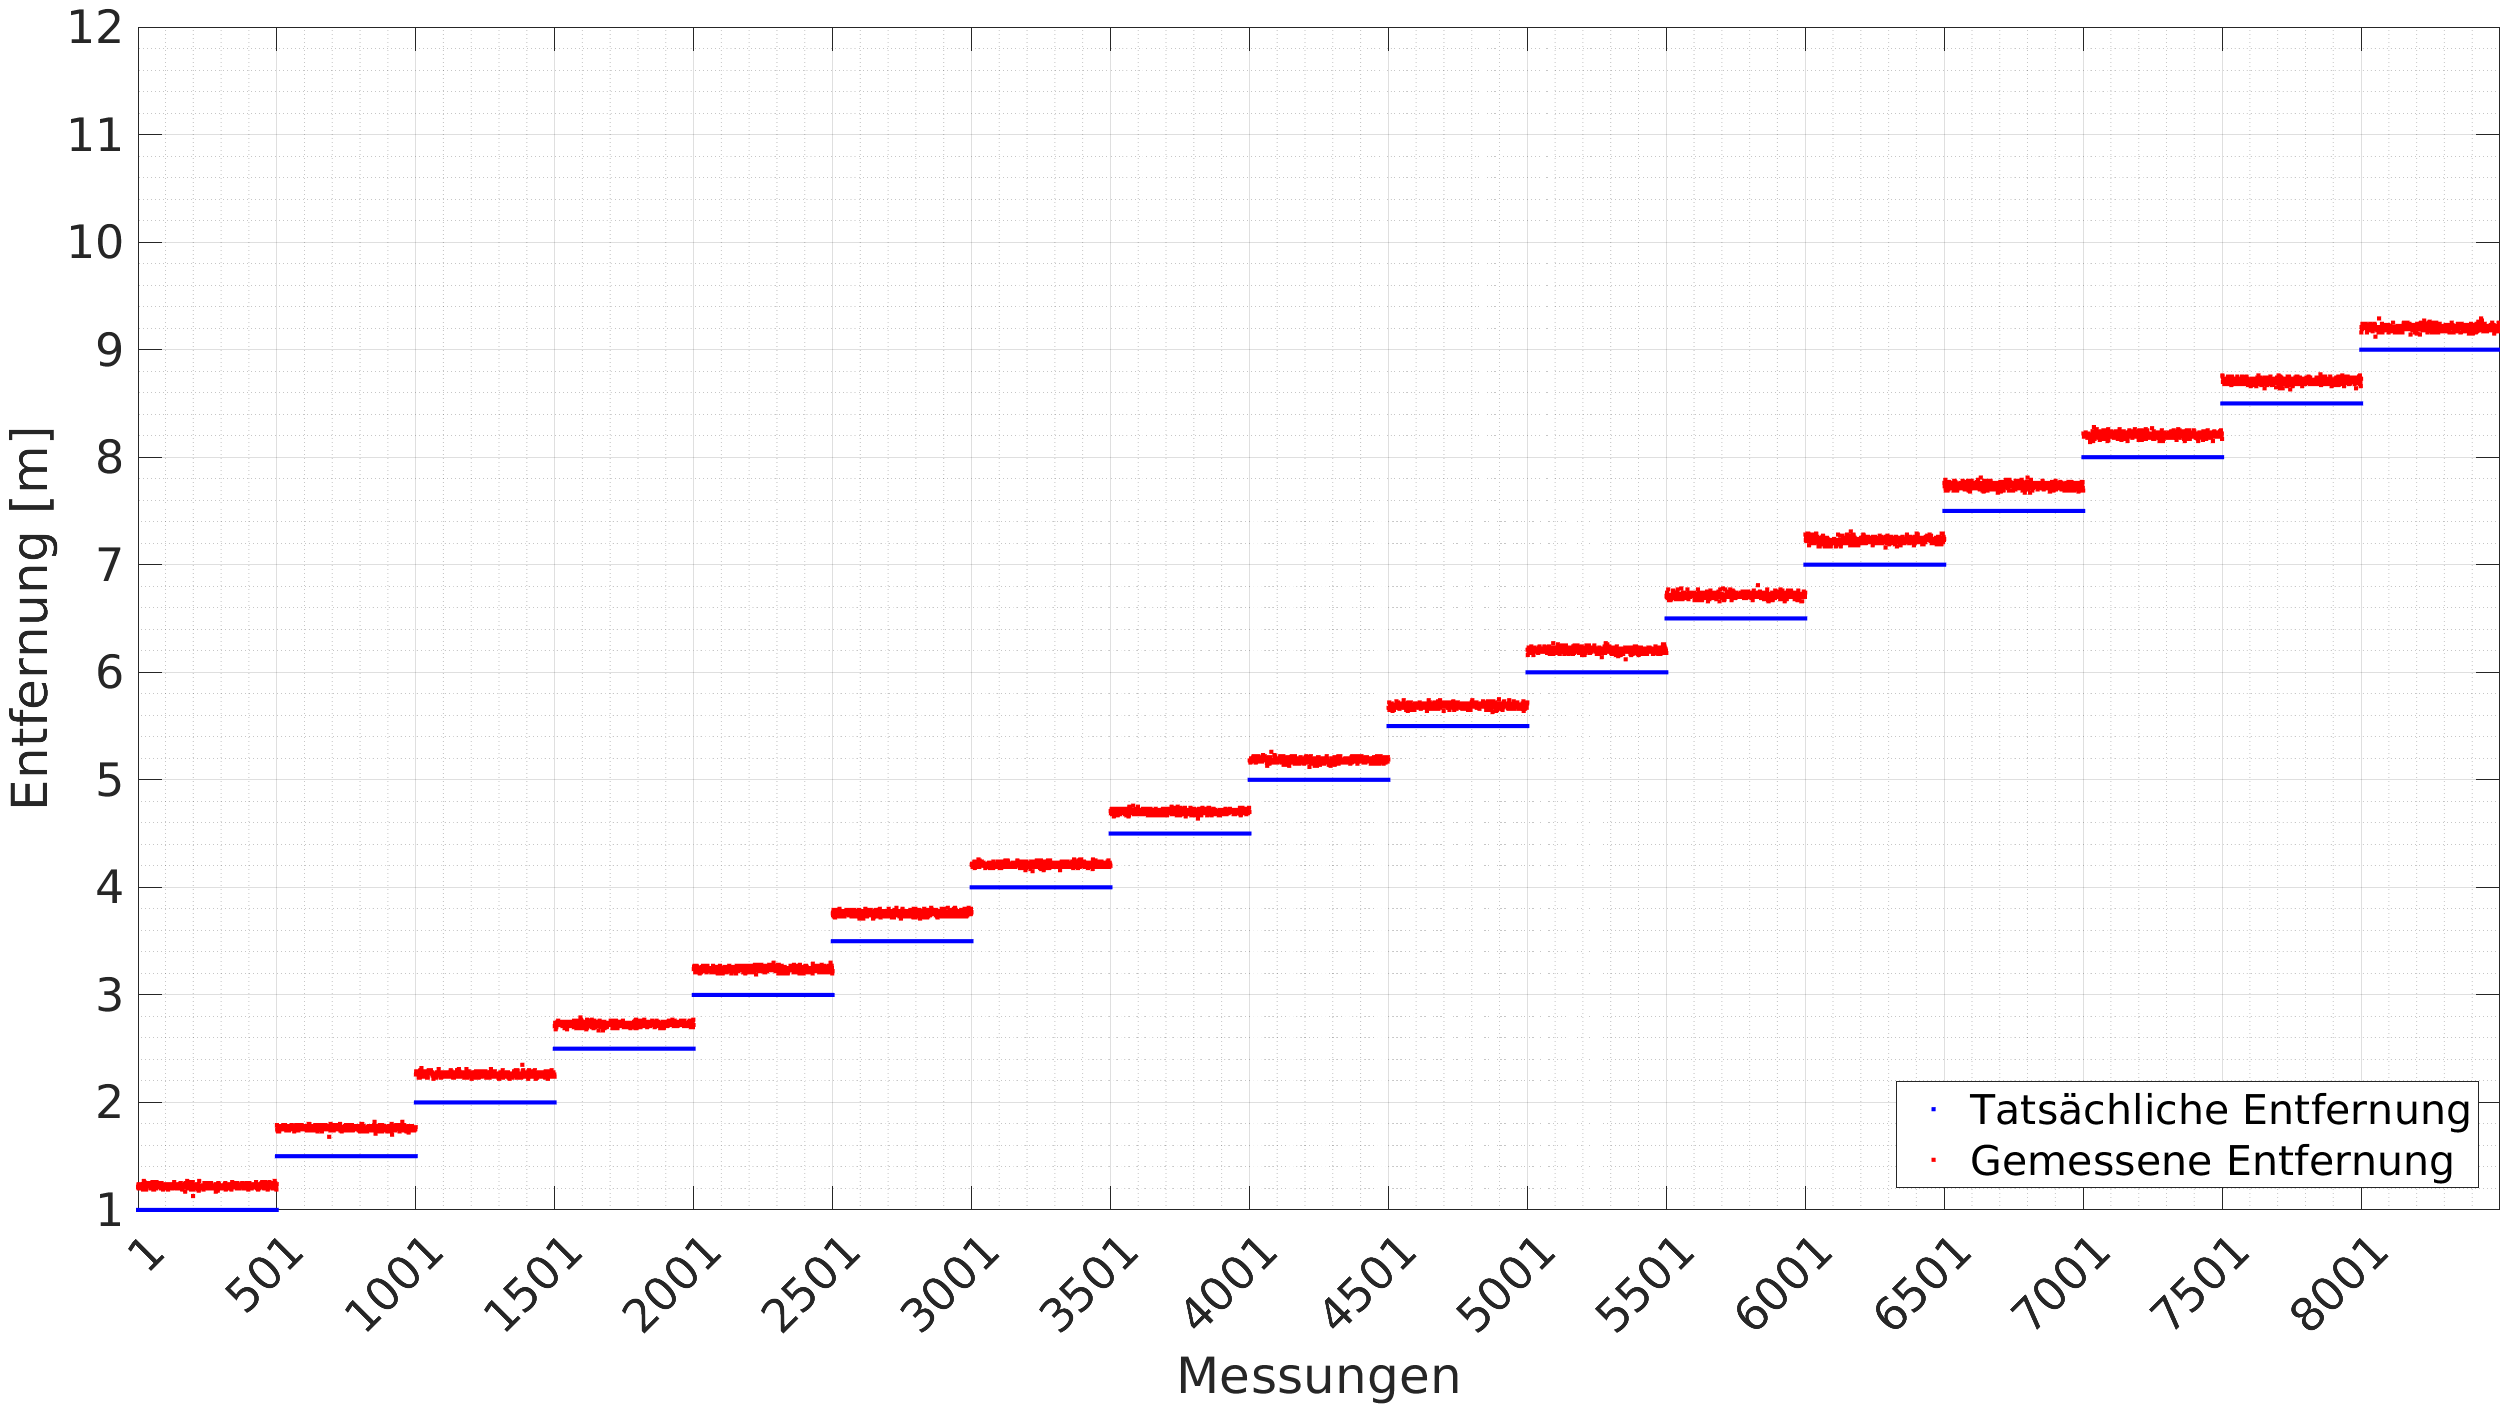
\includegraphics[width=\linewidth]{entfernungsmessung_2018_01_20_los}
%			\caption{LoS}
		\end{subfigure}
		\hfill
		\begin{subfigure}[t]{0.47\linewidth}
			\centering
			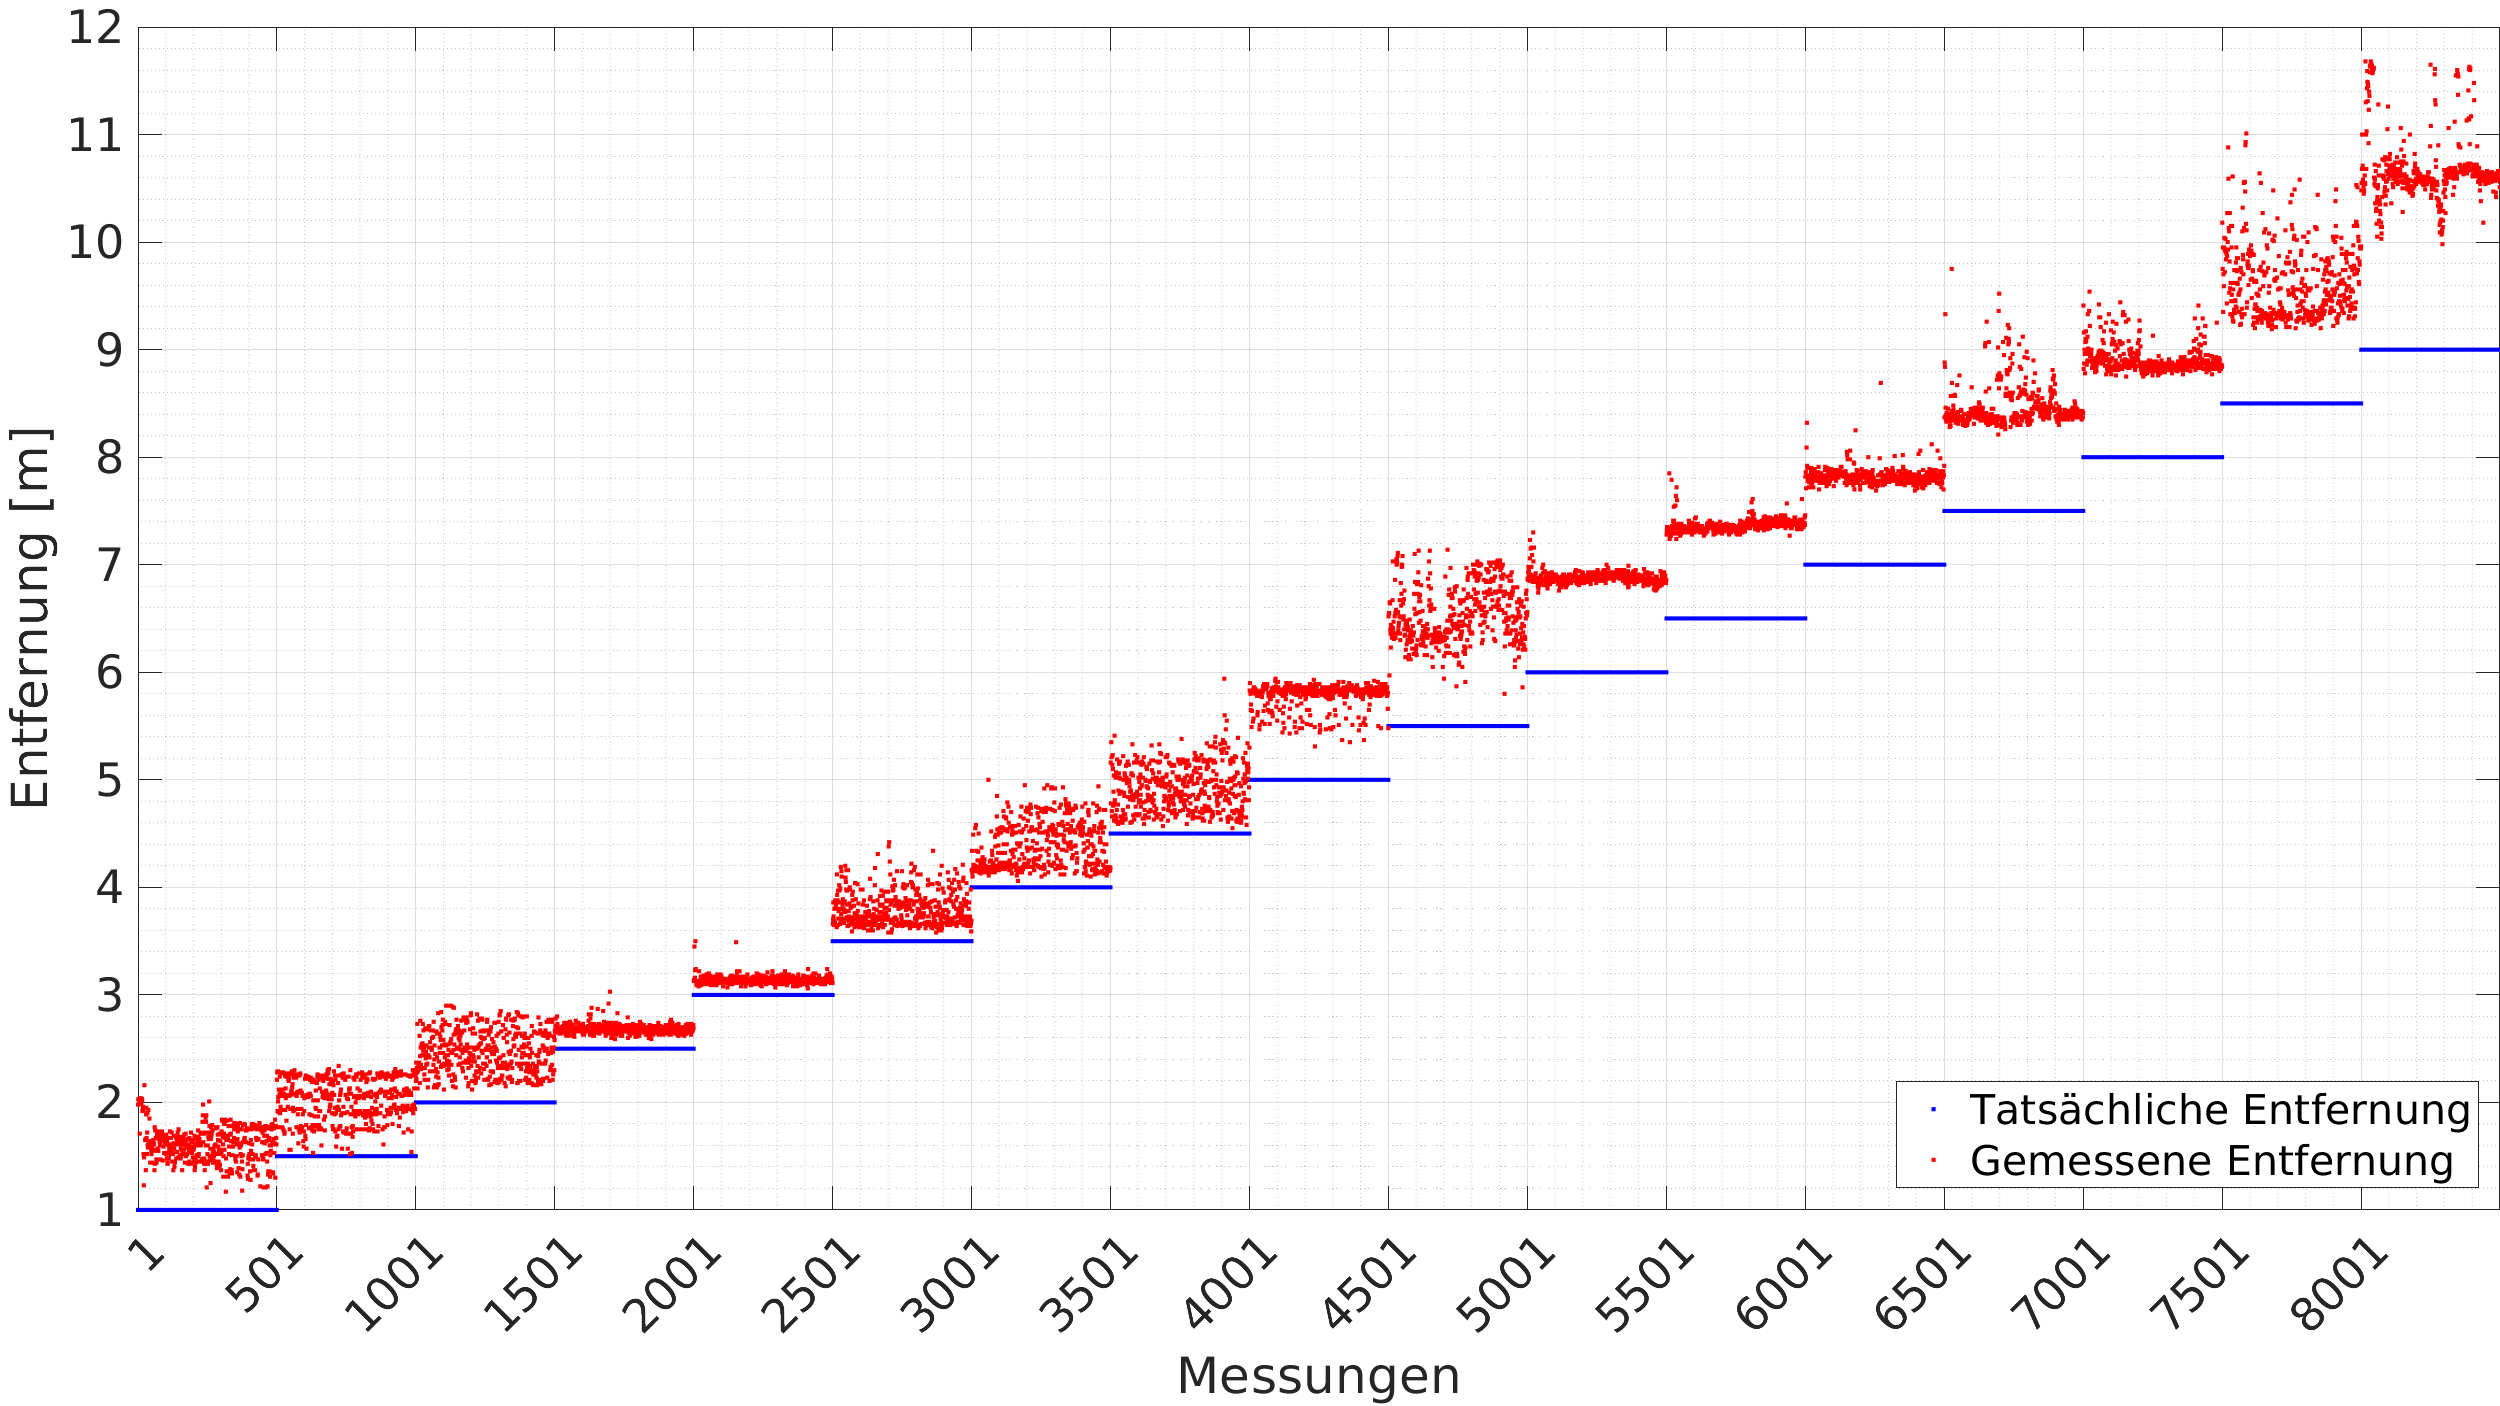
\includegraphics[width=\linewidth]{entfernungsmessung_2018_01_20_nlos_water}
%			\caption{NLoS mit Wasser.}
		\end{subfigure}
		\par
		\bigskip
		\begin{subfigure}[t]{0.47\linewidth}
			\centering
			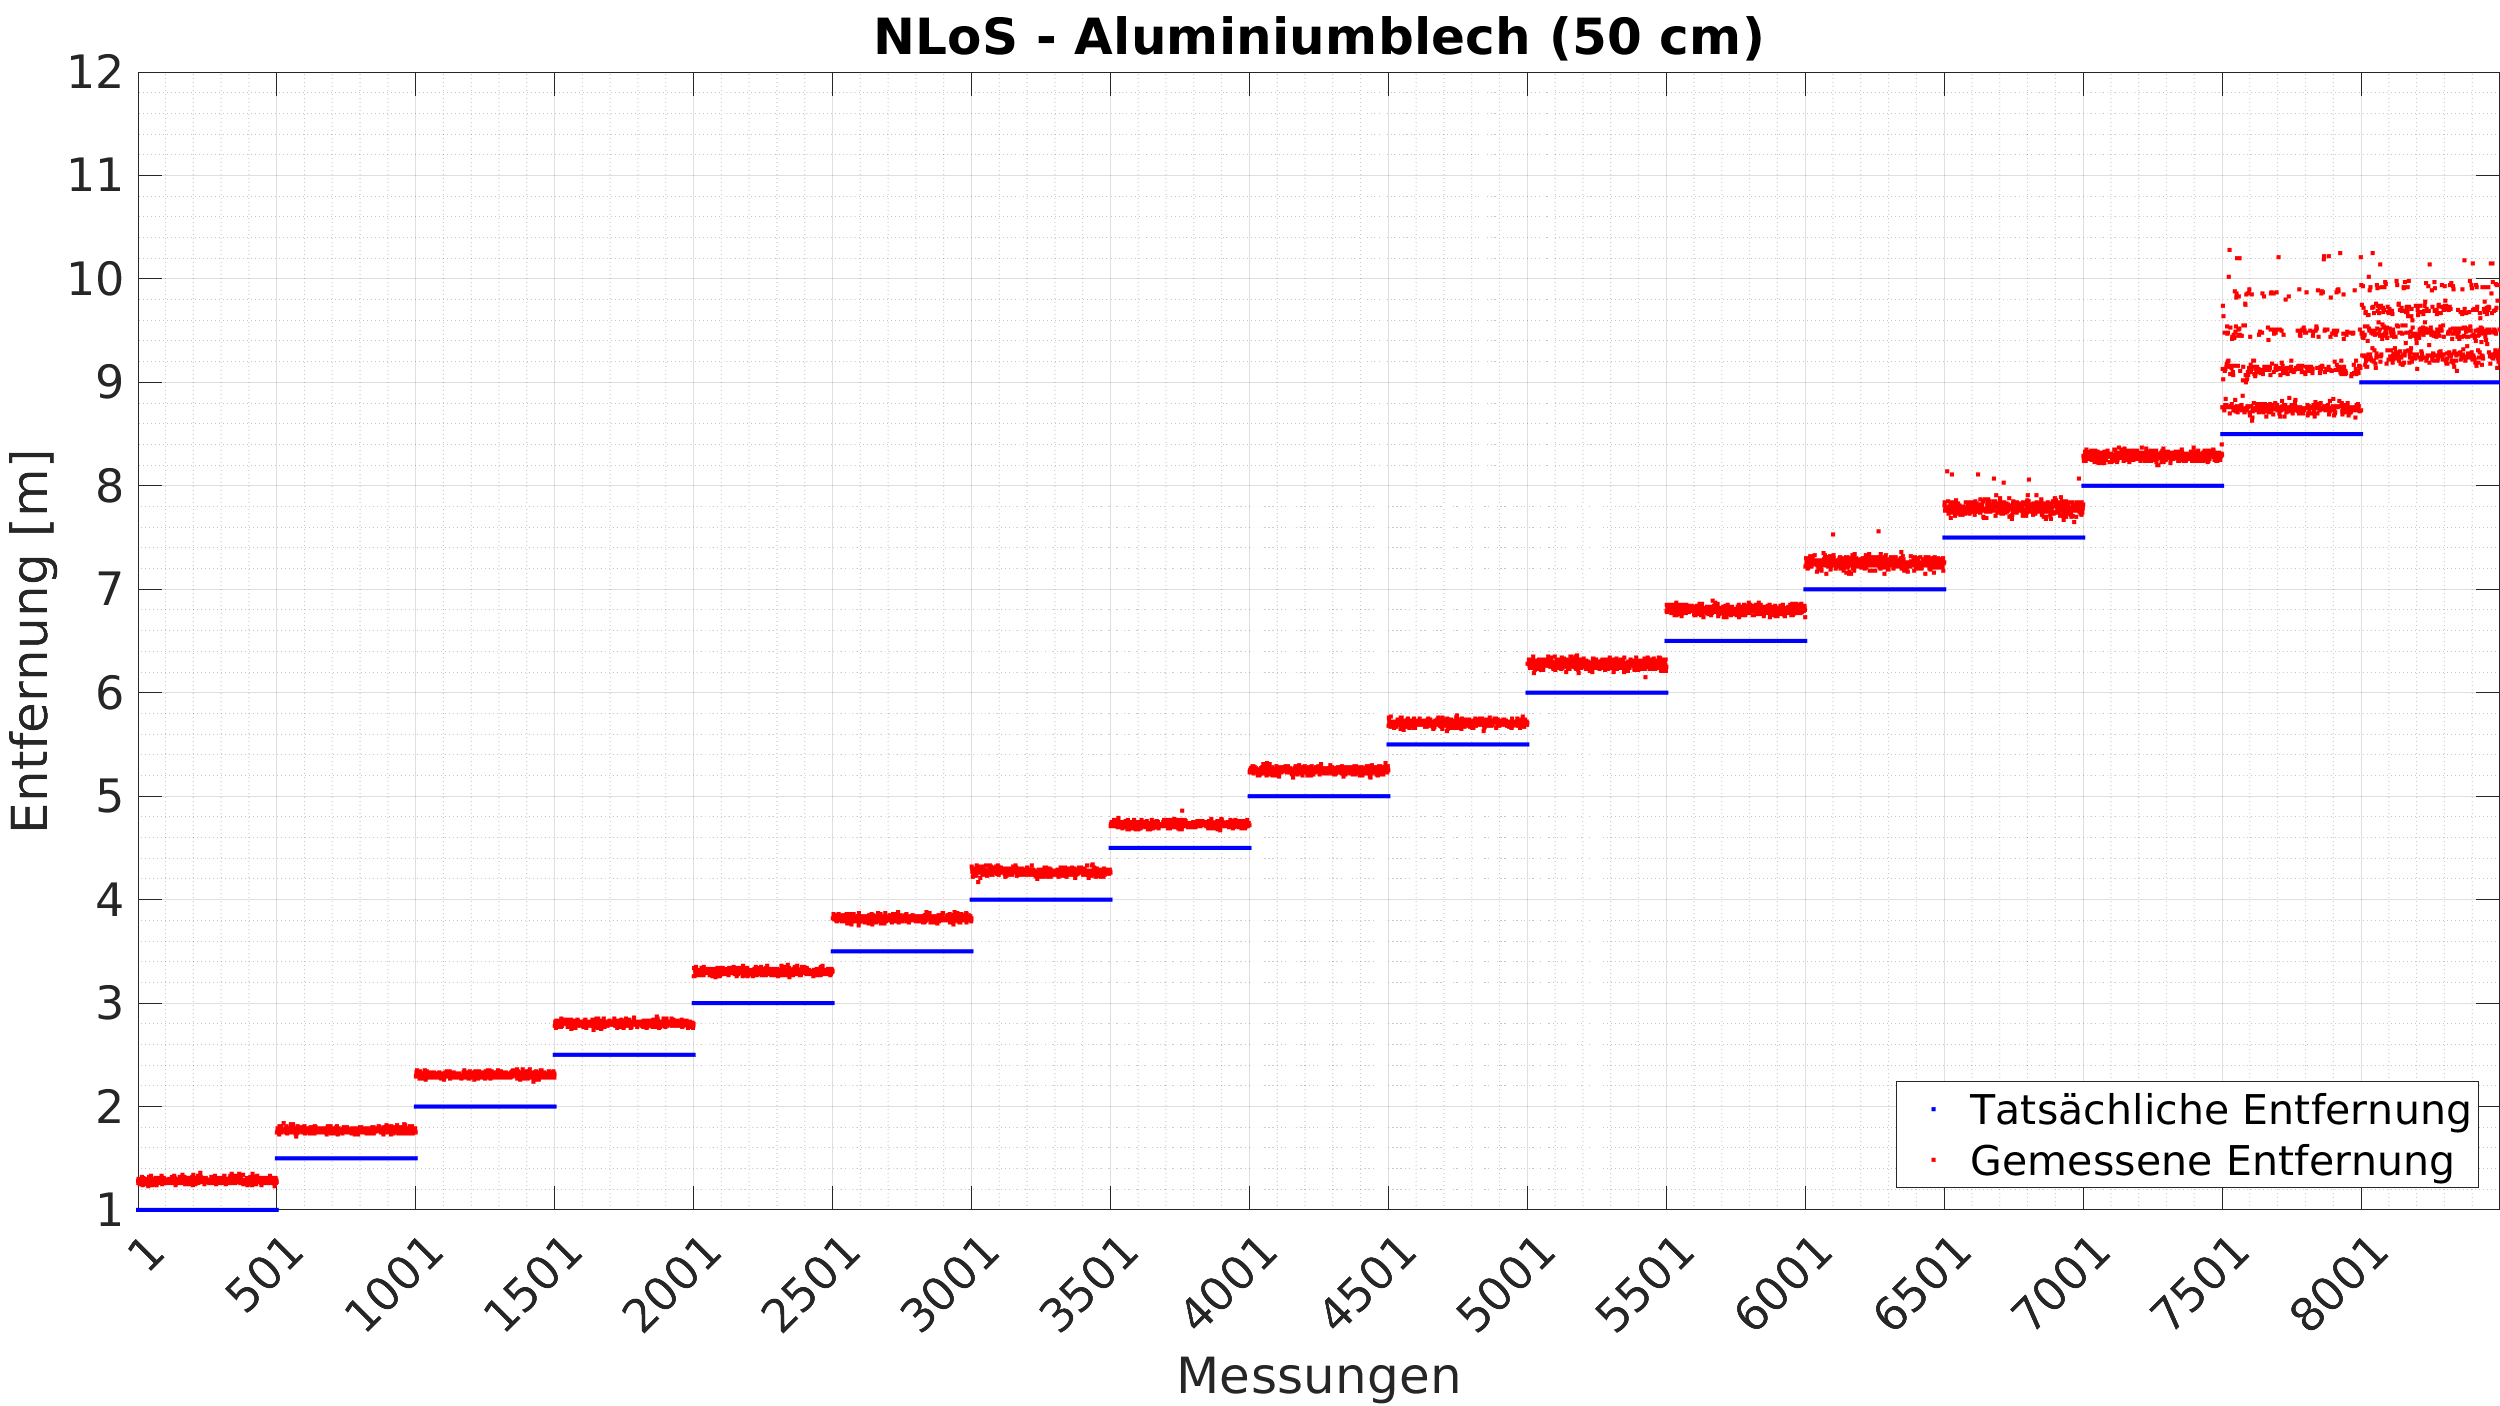
\includegraphics[width=\linewidth]{entfernungsmessung_2018_01_20_nlos_metal}
%			\caption{NLoS mit einem Aluminiumblech (\SI{50}{\centi\meter})}
		\end{subfigure}
		\hfill
		\begin{subfigure}[t]{0.47\linewidth}
			\centering
			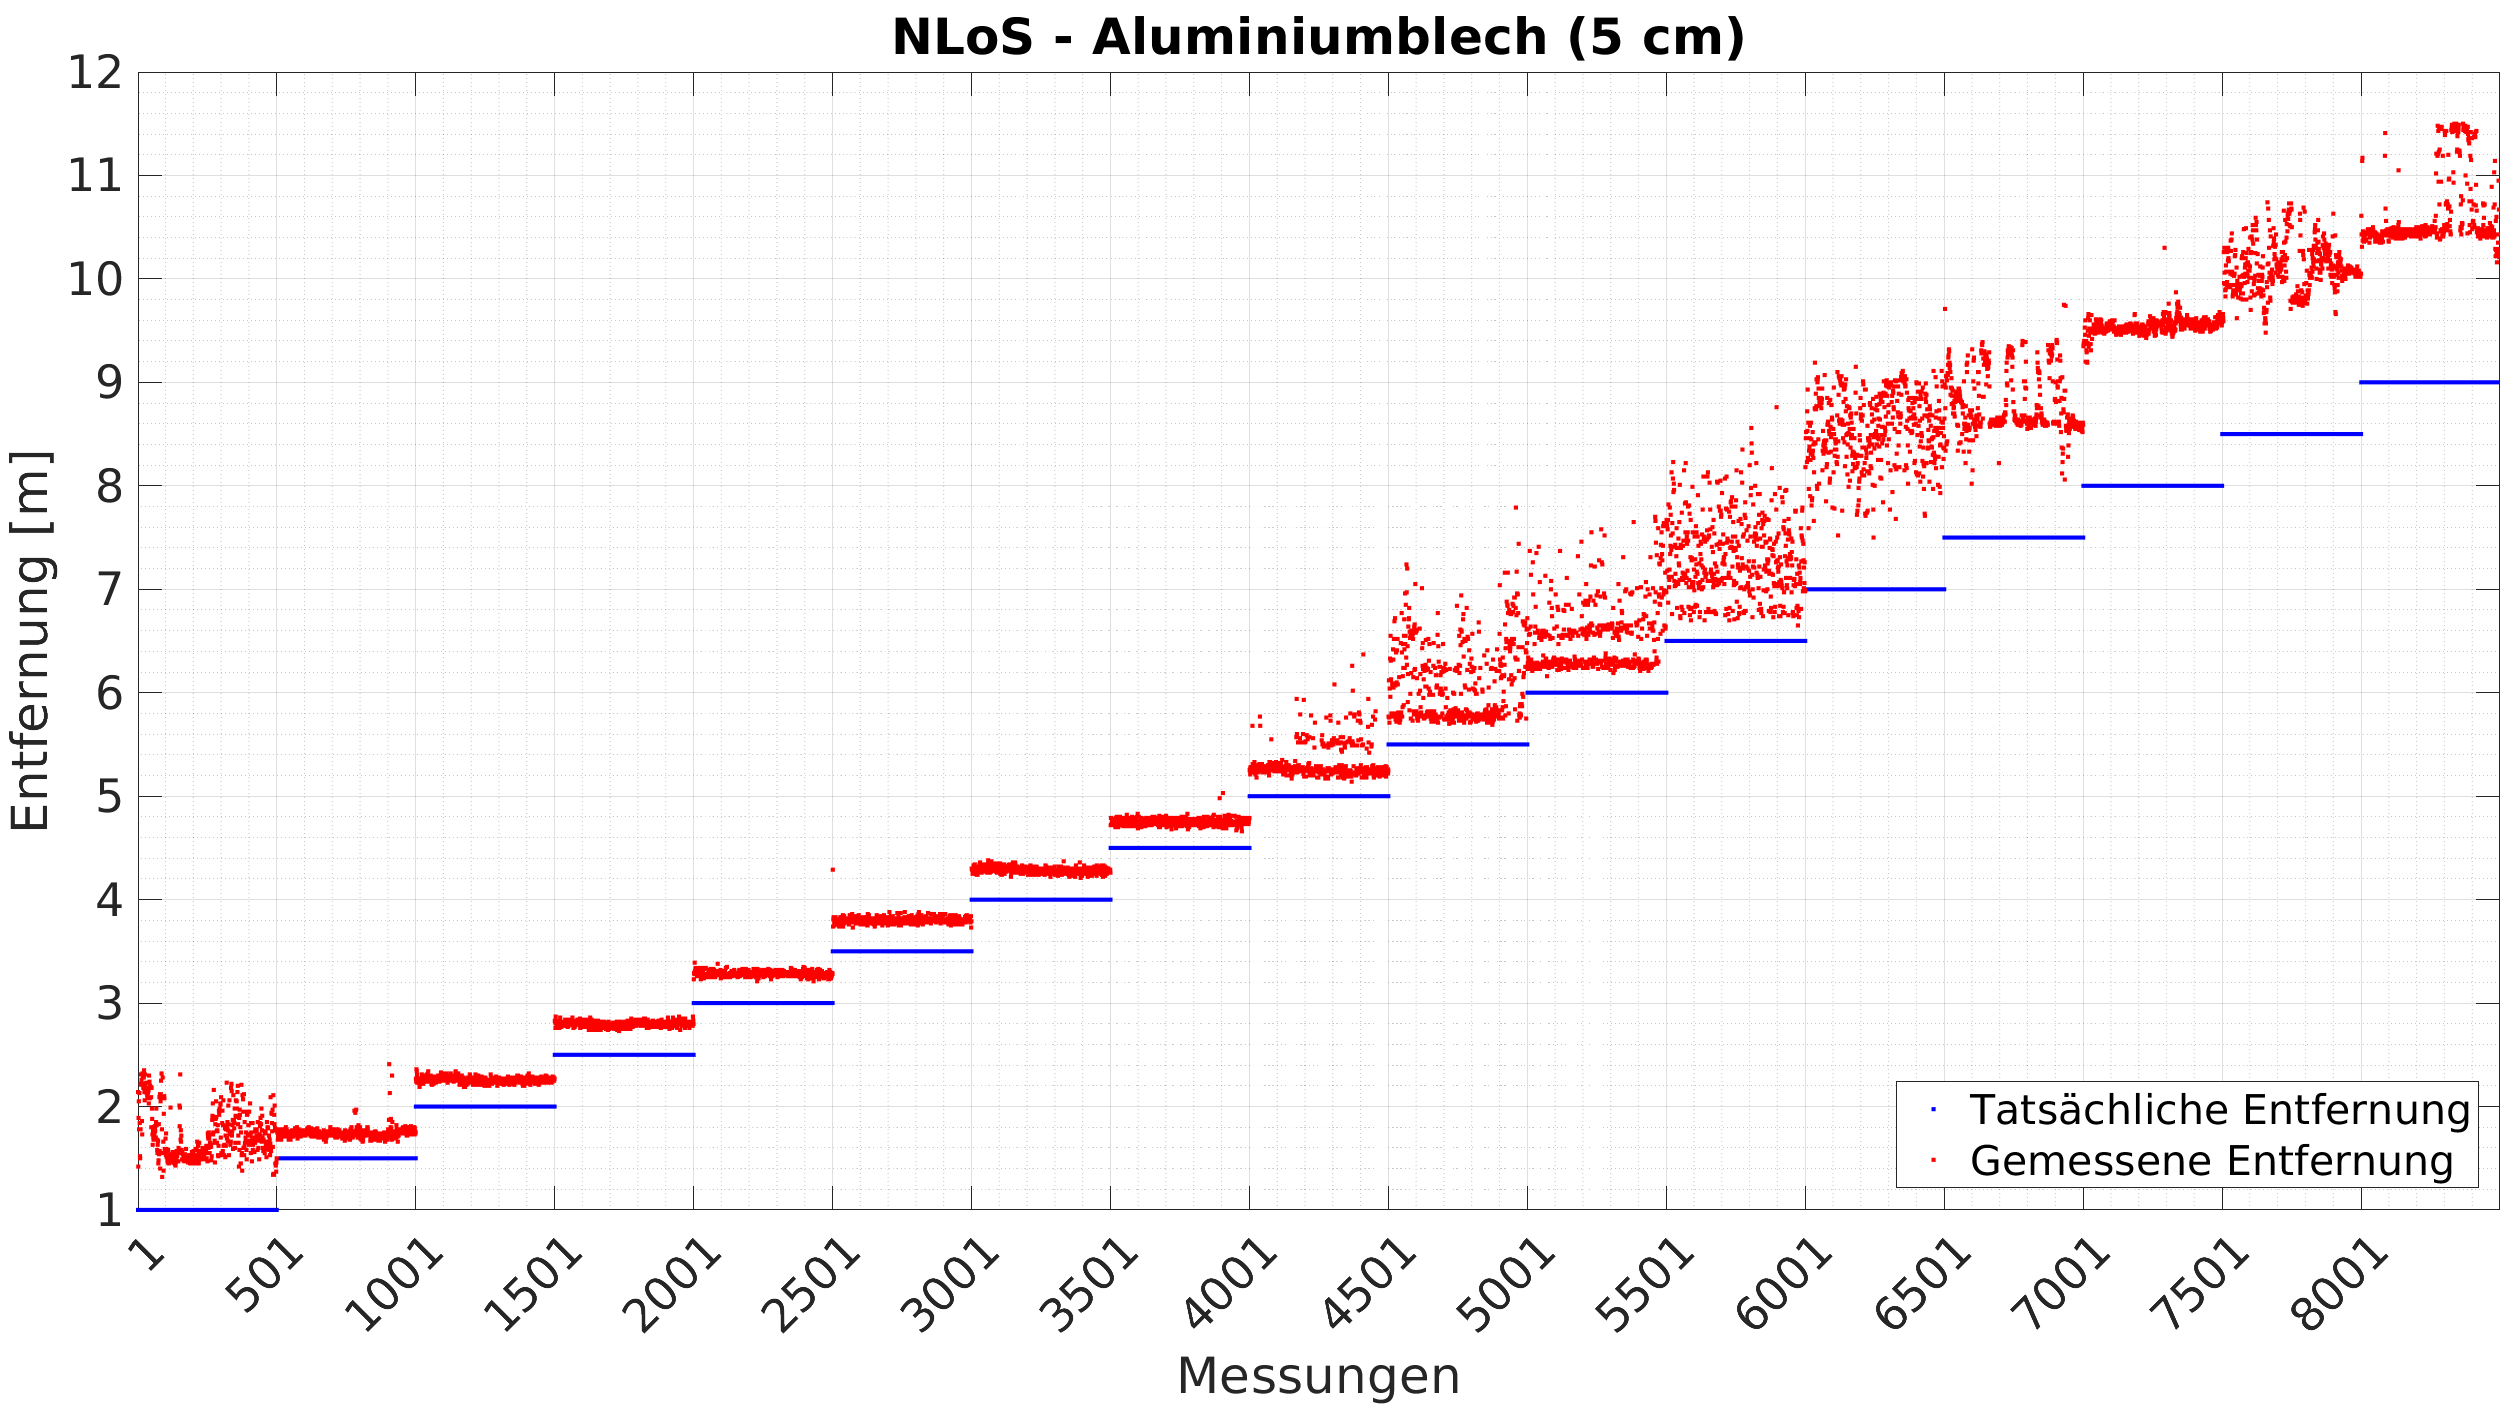
\includegraphics[width=\linewidth]{entfernungsmessung_2018_01_20_nlos_metal2}
%			\caption{NLoS mit einem Aluminiumblech (\SI{5}{\centi\meter})}
		\end{subfigure}
	\end{figure}
\end{frame}


%%%%%%%%%%%%%%%%%%%%%%%%%%%%%%%%%%%%%%%%%%%%%%%%%%%%%%%%%%%%%%%%%%%%%%%%%%%%%%%%
%
% 
%
%%%%%%%%%%
\part{Range-Only SLAM}


%%%%%%%%%%%%%%%%%%%%%%%%%%%%%%%%%%%%%%%%%%%%%%%%%%%%%%%%%%%%%%%%%%%%%%%%%%%%%%%%
%
%	- FastSLAM
%		- http://slideplayer.com/slide/4547004/
%		- FastSLAM Update Action
% 	- Rao-Blackwellized Partikelfilter
%		- Problem mit Parikelfilter und großem Zustandsraum
% 		- Kernidee
%	- \cite{thrun2005probabilistic}
%		- Probabilistic robotics
%	- todo
%		- Das andere Bild für den RBPF verwenden.
%
%%%%%%%%%%
\begin{frame}{Theorie (1/3)\\Partikel Filter}
	\begin{columns}
		\begin{column}{0.5\linewidth}
			\parbox[c][.7\textheight][c]{\columnwidth}
			{
				\includegraphics<1>[width=\linewidth]{ekf_slam_fig_10_3}
				\includegraphics<2>[width=\linewidth]{fast_slam_particle_representation}
			}
		\end{column}
		\begin{column}{0.5\linewidth}
			\begin{itemize}
				\item<1-> EKF SLAM
					\begin{itemize}
						\item Kombinierter Zustandsvektor
					\end{itemize}
				\item<2-> PF SLAM
					\begin{itemize}
						\item Aufspaltung des Zustandsvektor
						\item Rao-Blackwellized Partikel Filter
						\item FastSLAM
					\end{itemize}
			\end{itemize}
		\end{column}
	\end{columns}
\end{frame}


%%%%%%%%%%%%%%%%%%%%%%%%%%%%%%%%%%%%%%%%%%%%%%%%%%%%%%%%%%%%%%%%%%%%%%%%%%%%%%%%
%
%	- \cite{blanco2008pure}
%		- A pure probabilistic approach to range-only SLAM
%	- decouple the estimation of the robot poses and the map (rbpf)
%	- robot path is sample based
%	- for each beacon that is observed for the first time, we add a new auxiliary particle filter to each one of the rbpf samples.
%	- the auxiliary pf will eventually converge from the initial circular shape towards a small Gaussian-like shape, and at this moment it will be raplaced by a standard EKF.
%	- the location of the beacon is approximated by a set of N samples m^[i,k] with weights \beta^[i,k] for k=1..N.
%	- Initialize the Monte Carlo representation of the beacon density by drawing samples m^[i,k] along the circle centered at x_t^[i] at any direction in the whole 360° range and at a distance of z_t plus the additive random noise. (assign them with equal inital weights)
%	- we drop particles with weights below 10^-5 times the hightest weight.
%
%%%%%%%%%%
\begin{frame}{Theorie (2/3)\\Monte Carlo Partikel Filter mit Hilfspartikel Filter}
	\begin{columns}
		\column{0.5\linewidth}
			\begin{overlayarea}{\textwidth}{.7\textheight}
				\only<1>
				{
					\begin{figure}
						\centering
						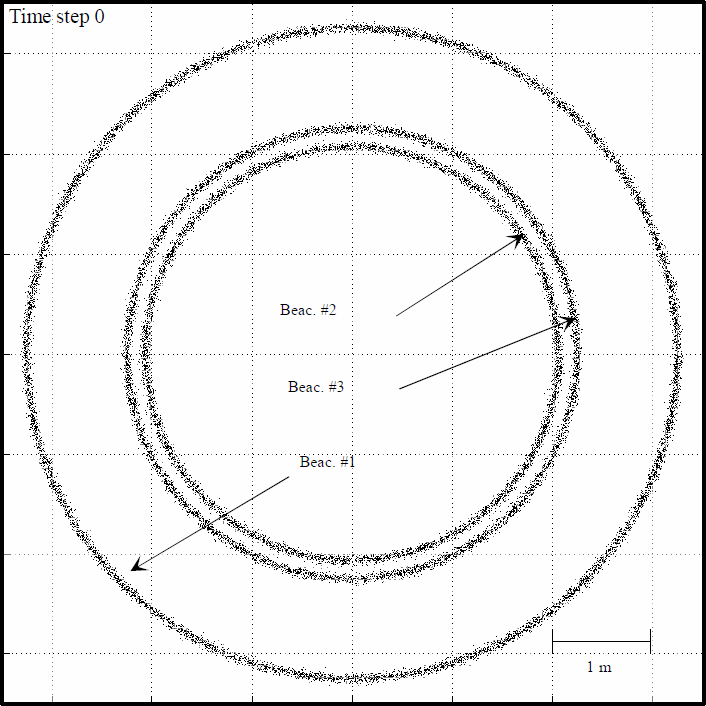
\includegraphics[width=\linewidth]{blanco2008pure_fig3e}
						\caption{\cite{blanco2008pure}}
					\end{figure}
				}
				\only<2>
				{
					\begin{figure}
						\centering
						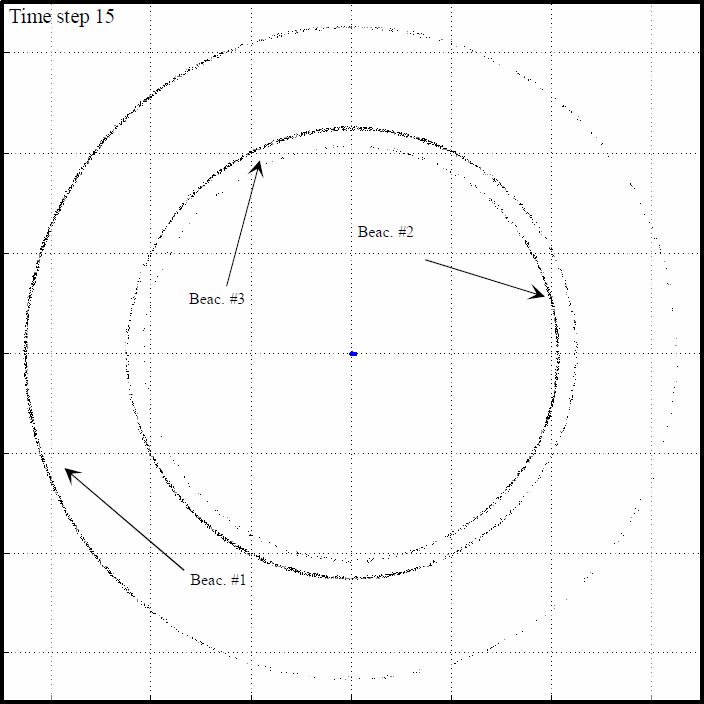
\includegraphics[width=\linewidth]{blanco2008pure_fig3f}
						\caption{\cite{blanco2008pure}}
					\end{figure}
				}
				\only<3>
				{
					\begin{figure}
						\centering
						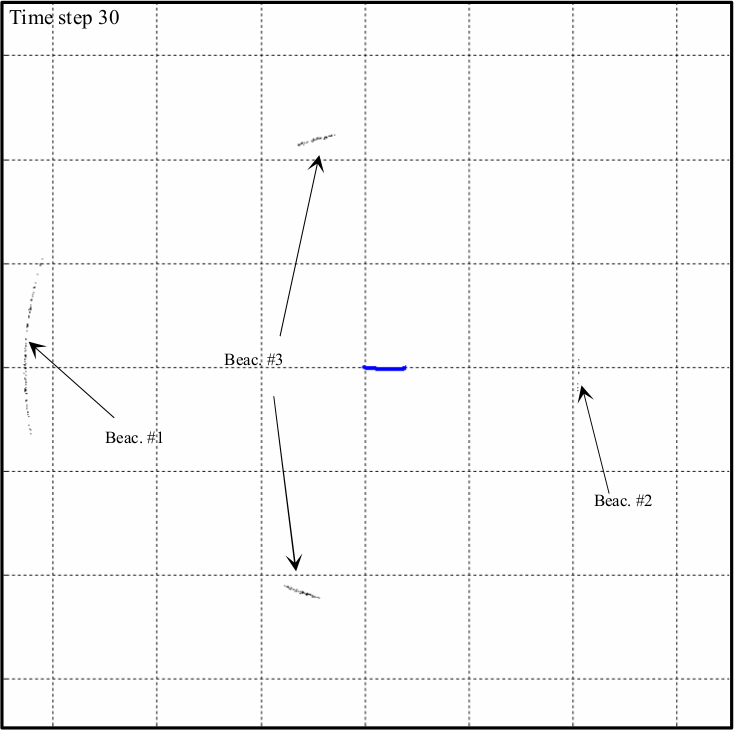
\includegraphics[width=\linewidth]{blanco2008pure_fig3g}
						\caption{\cite{blanco2008pure}}
					\end{figure}
				}
				\only<4>
				{
					\begin{figure}
						\centering
						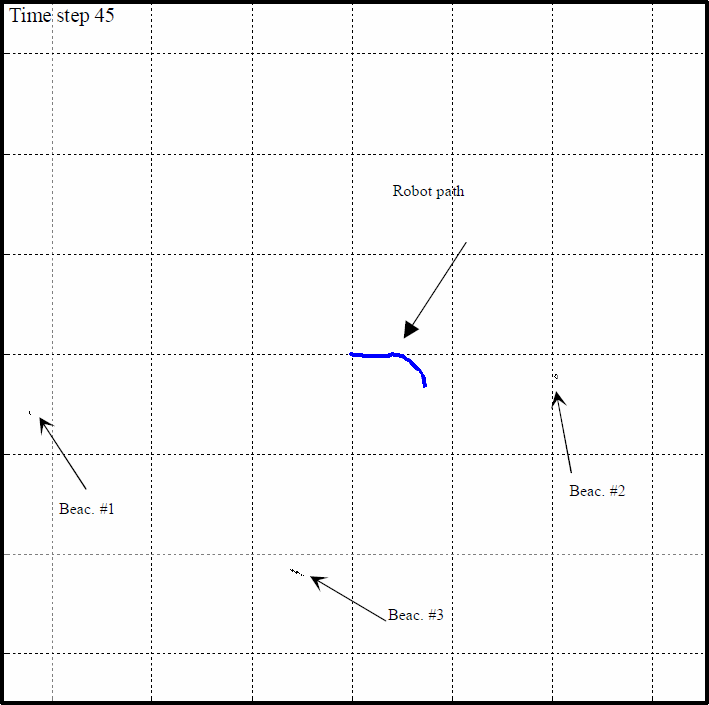
\includegraphics[width=\linewidth]{blanco2008pure_fig3h}
						\caption{\cite{blanco2008pure}}
					\end{figure}
				}
			\end{overlayarea}		
		\column{0.5\linewidth}
			\begin{itemize}
				\item Hauptpartikel Filter
				\begin{itemize}
					\item Betrachung eines Partikels
				\end{itemize}
				\item Hilfspartikel Filter
				\begin{itemize}
					\item Pro UWB Modul
					\item Radiale Verteilung
					\item Gewicht pro Partikel
				\end{itemize}
				\item<4-> Nach der Konvergenz
				\begin{itemize}
					\item Umwandung in einen EKF
				\end{itemize}
			\end{itemize}
	\end{columns}
\end{frame}



%%%%%%%%%%%%%%%%%%%%%%%%%%%%%%%%%%%%%%%%%%%%%%%%%%%%%%%%%%%%%%%%%%%%%%%%%%%%%%%%
%
%	- https://www.mrpt.org/tutorials/slam-algorithms/rangeonly_slam/
%	- \cite{blanco2008efficient}
%		- Efficient probabilistic range-only SLAM
%	- Kugelkoordinaten
%		- 3 Einheitsvektoren (1x Radial, 2x Tangential)
%		- Stachlige Kugel?!
%
%%%%%%%%%%
\begin{frame}
	\frametitle{Theorie (3/3)\\Monte Carlo Partikel Filter mit Sum of Gaussian}
	\begin{columns}
		\column{0.5\linewidth}
			\begin{overlayarea}{\textwidth}{.5\textheight}
				\only<1>
				{
					\begin{figure}
						\centering
						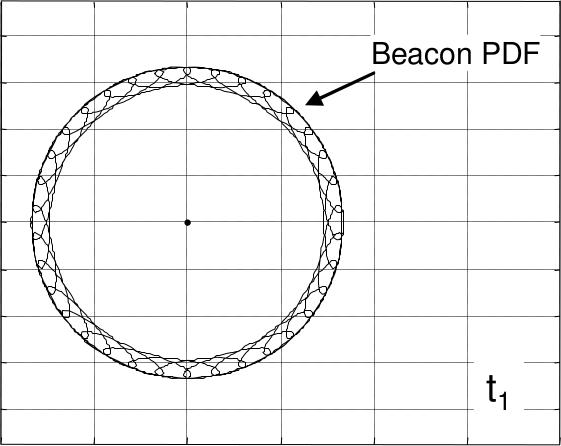
\includegraphics[width=\linewidth]{blanco2008efficient_fig3_1}
						\caption{\cite{blanco2008efficient}}
					\end{figure}
				}
				\only<2>
				{
					\begin{figure}
						\centering
						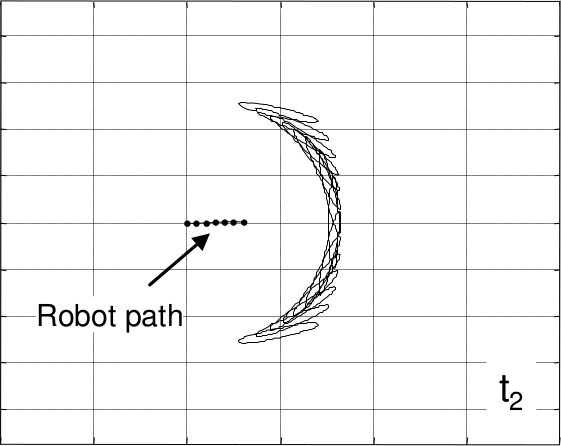
\includegraphics[width=\linewidth]{blanco2008efficient_fig3_2}
						\caption{\cite{blanco2008efficient}}
					\end{figure}
				}
				\only<3>
				{
					\begin{figure}
						\centering
						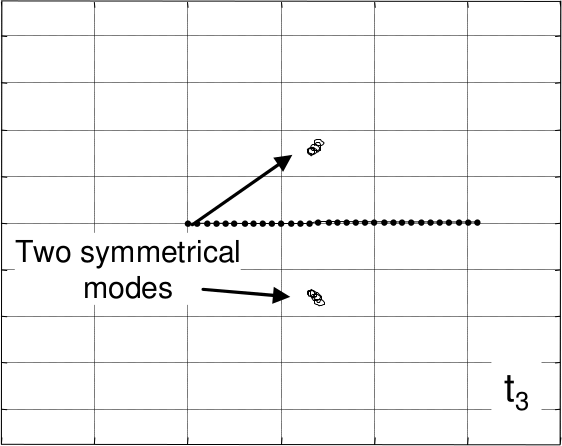
\includegraphics[width=\linewidth]{blanco2008efficient_fig3_3}
						\caption{\cite{blanco2008efficient}}
					\end{figure}
				}
				\only<4>
				{
					\begin{figure}
						\centering
						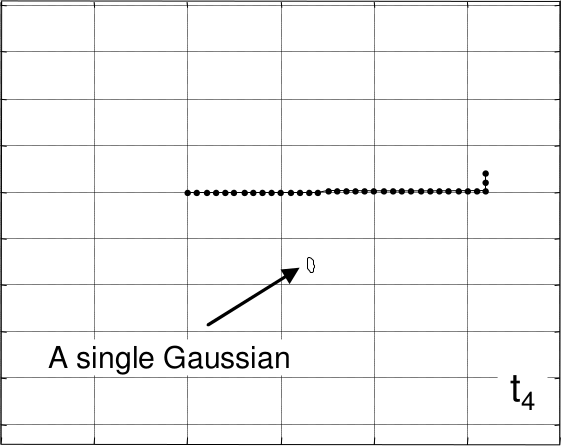
\includegraphics[width=\linewidth]{blanco2008efficient_fig3_4}
						\caption{\cite{blanco2008efficient}}
					\end{figure}
				}
			\end{overlayarea}
		\column{0.5\linewidth}
			\begin{itemize}
				\item Hauptpartikel Filter
				\begin{itemize}
					\item Betrachung eines Partikels
				\end{itemize}
				\item Sum of Gaussian (SOG)
				\begin{itemize}
					\item Radial angeordnete Normalverteilungen
					\item Gewicht pro Normalverteilung
					\item Pro UWB Modul
				\end{itemize}
				\item<4-> Nach der Konvergenz
				\begin{itemize}
					\item Umwandung in einen EKF
				\end{itemize}
			\end{itemize}
	\end{columns}
\end{frame}


%%%%%%%%%%%%%%%%%%%%%%%%%%%%%%%%%%%%%%%%%%%%%%%%%%%%%%%%%%%%%%%%%%%%%%%%%%%%%%%%
%
%	- Warum ist die Odometrie so wichtig?
%	- Wie bin ich an die Ground Truth Trajektorie gekommen?
%	- /.../bachelor-thesis/auswertungen/trajectory/auswertung.m
%
%%%%%%%%%%
\begin{frame}{Odometrie}

	\begin{figure}
		\centering
		\begin{subfigure}{0.47\linewidth}
			\centering
			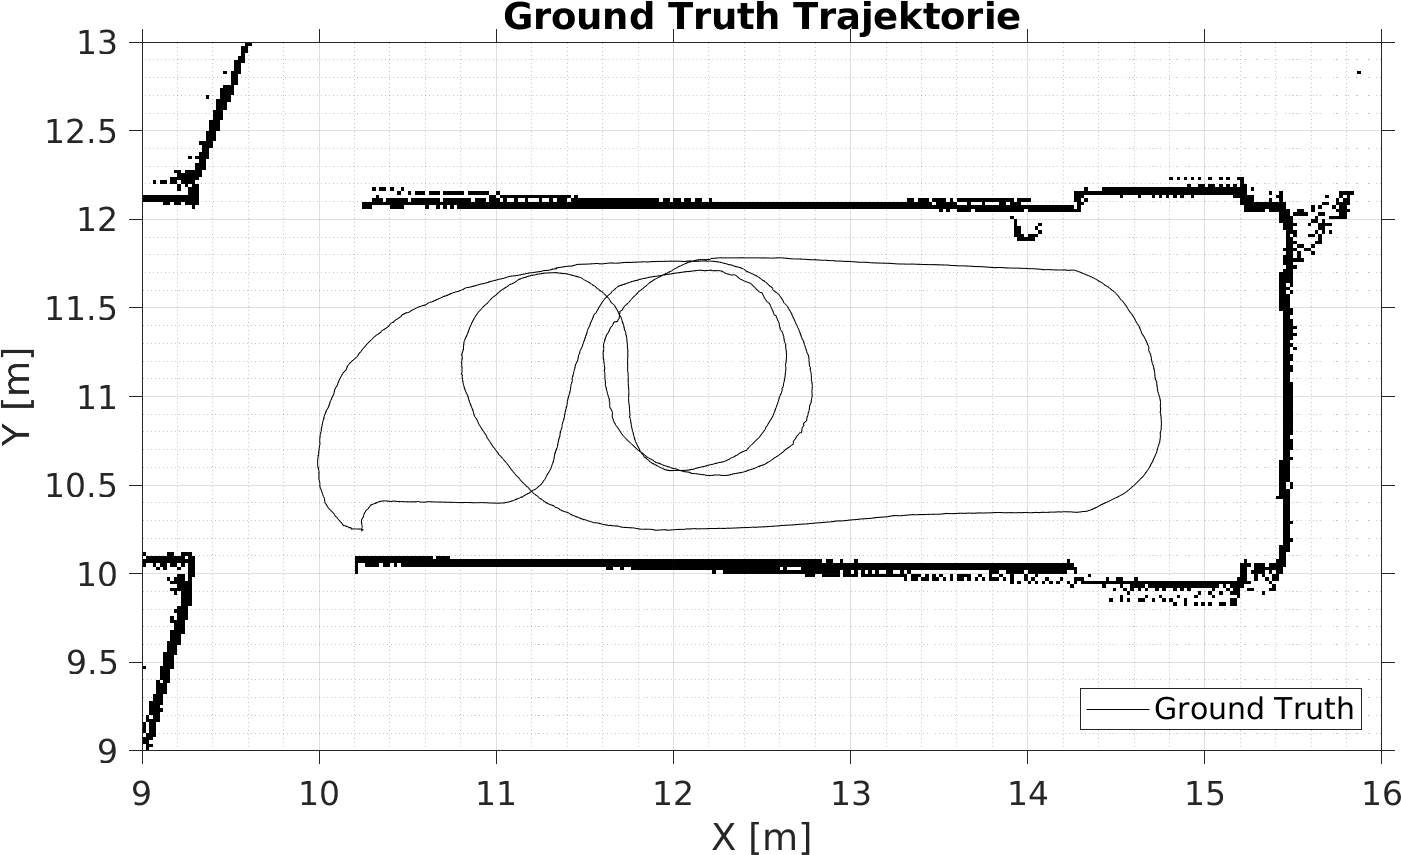
\includegraphics[width=\linewidth]{Record_2018-02-08-12-33-53_trajectory1}
			%\caption{Ground Truth}
		\end{subfigure}
		\hfill
		\begin{subfigure}{0.47\linewidth}
			\centering
			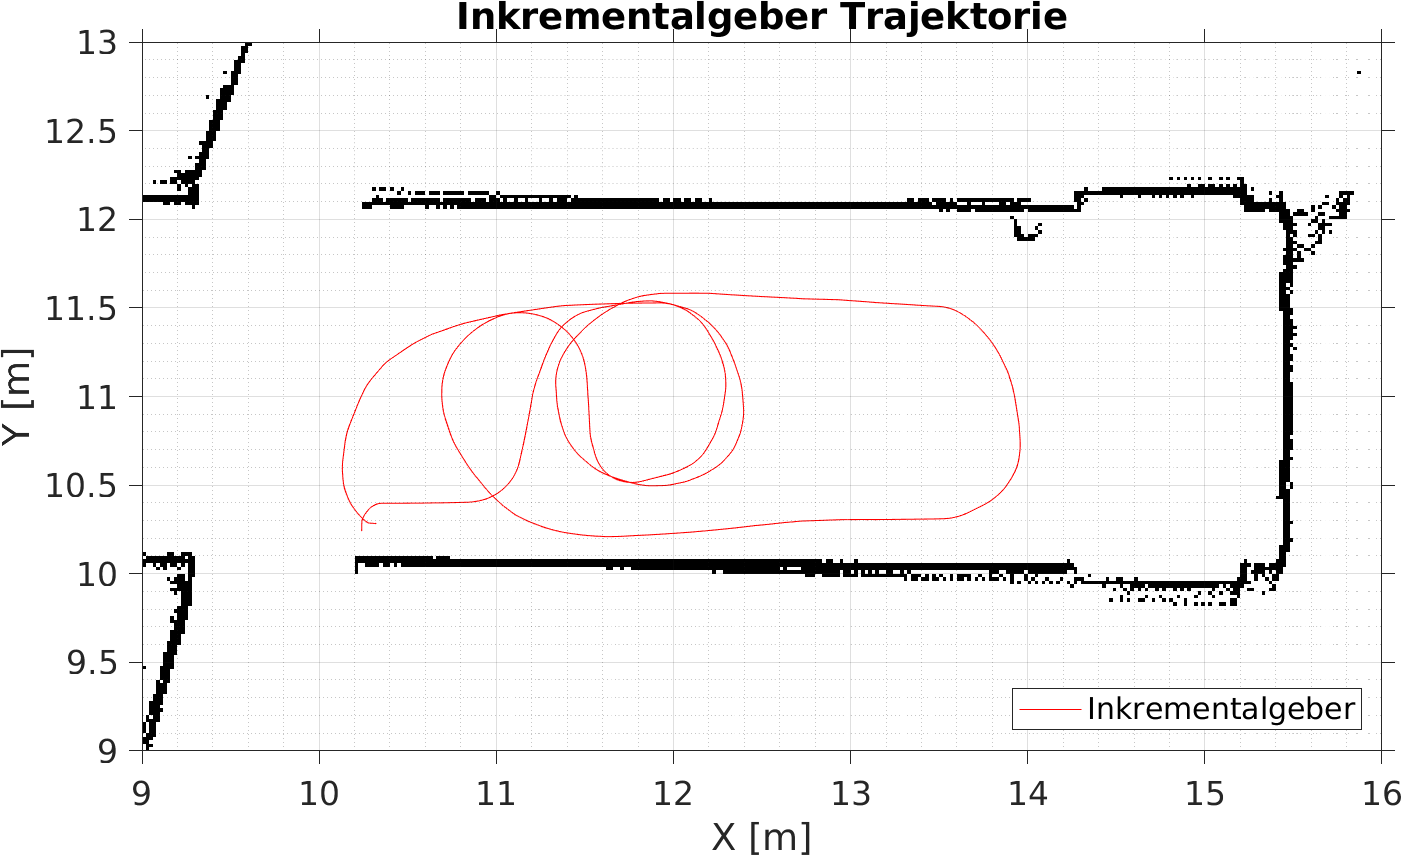
\includegraphics[width=\linewidth]{Record_2018-02-08-12-33-53_trajectory2}
			%\caption{Inkrementalgeber}
		\end{subfigure}
		\par
		\bigskip
		\begin{subfigure}{0.47\linewidth}
			\centering
			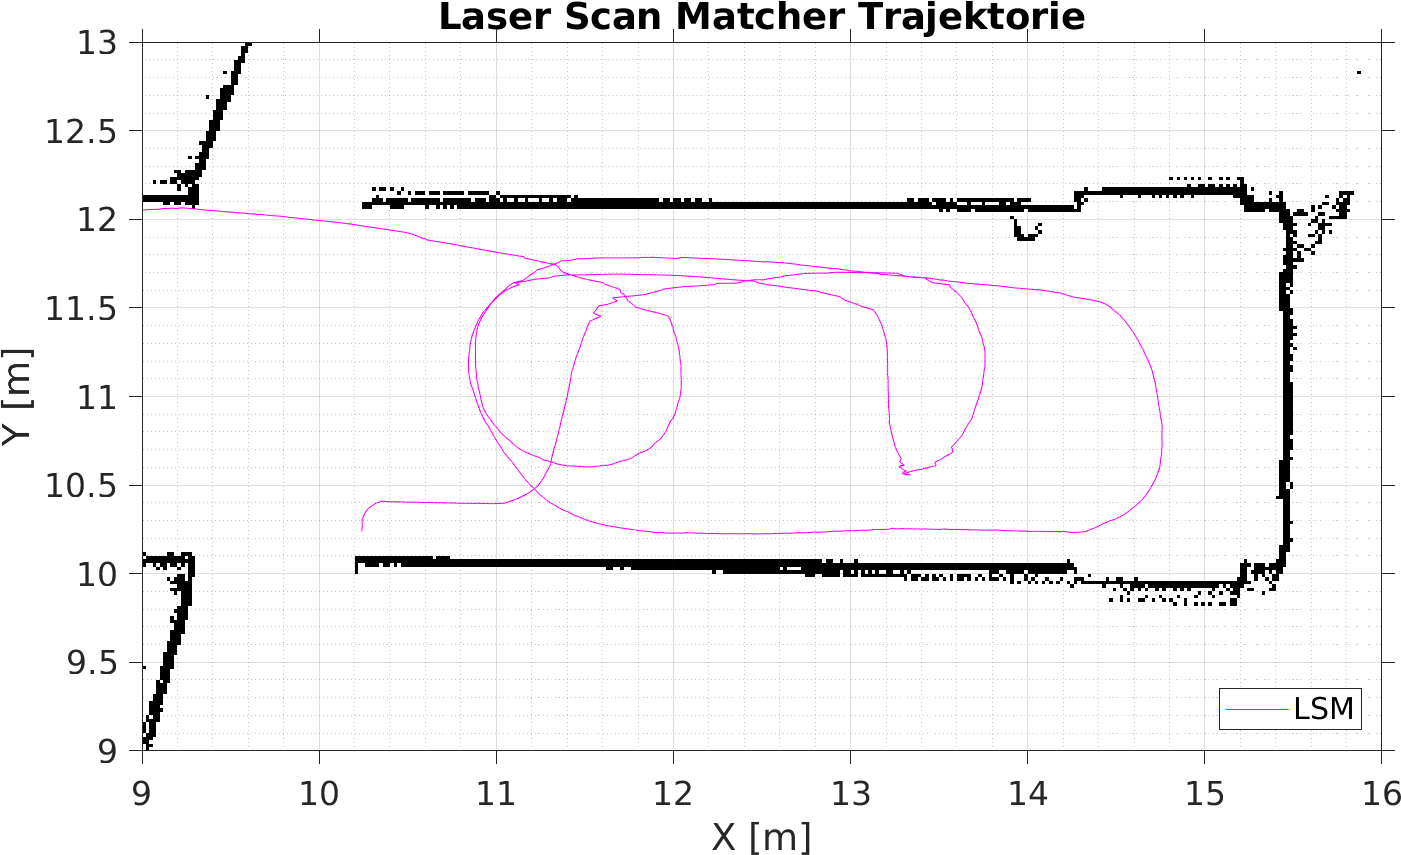
\includegraphics[width=\linewidth]{Record_2018-02-08-12-33-53_trajectory3}
			%\caption{Laser Scan Matcher}
		\end{subfigure}
		\hfill
		\begin{subfigure}{0.47\linewidth}
			\centering
			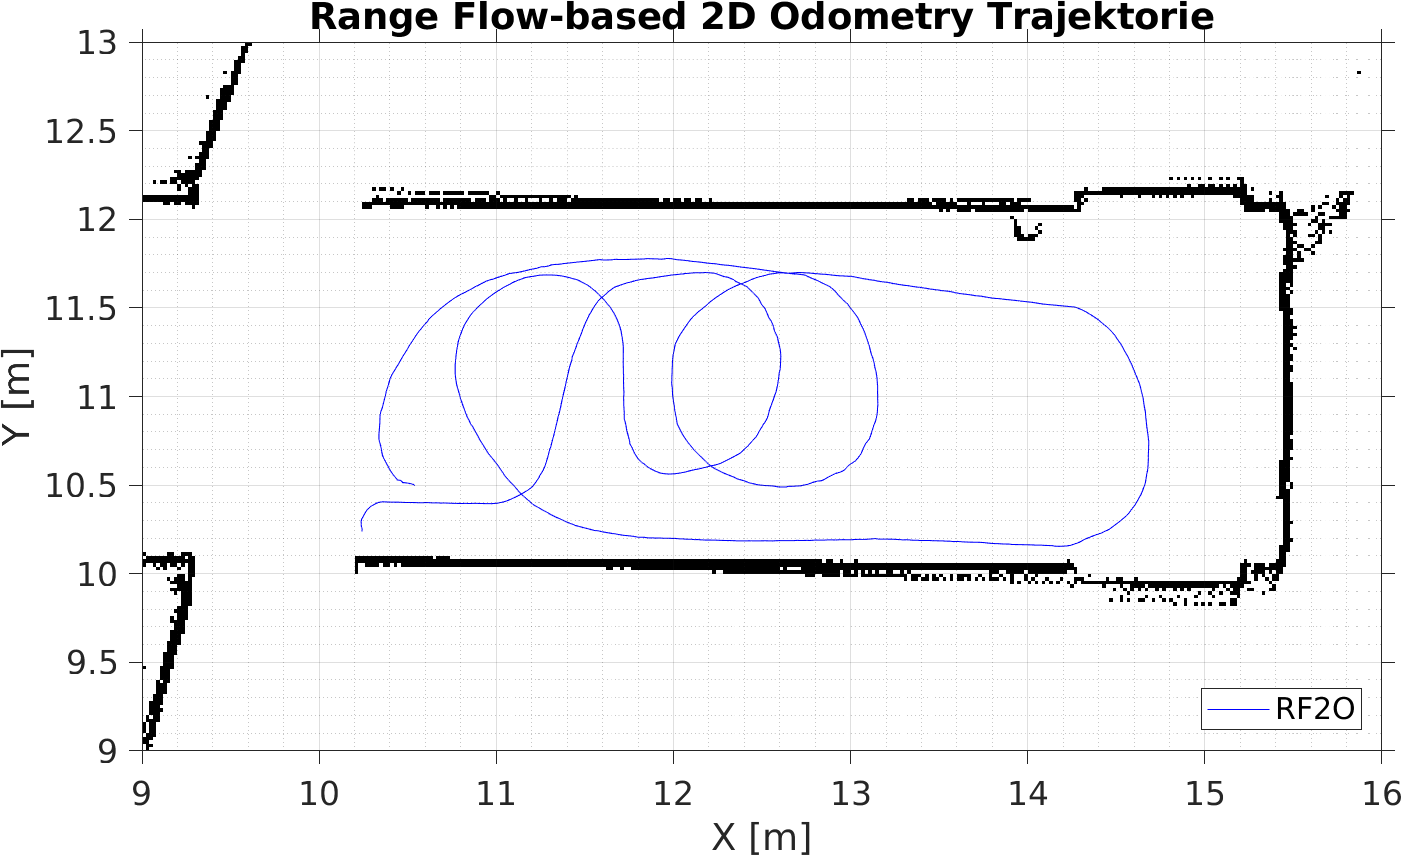
\includegraphics[width=\linewidth]{Record_2018-02-08-12-33-53_trajectory4}
			%\caption{Range Flow-based 2D Odometry}
		\end{subfigure}
	\end{figure}

\end{frame}


%%%%%%%%%%%%%%%%%%%%%%%%%%%%%%%%%%%%%%%%%%%%%%%%%%%%%%%%%%%%%%%%%%%%%%%%%%%%%%%%
%
%	- /.../bachelor-thesis/auswertungen/ro_slam_data/pose_diff.m
%
%%%%%%%%%%
\begin{frame}{Positionsschätzung der Roboterplattform}

	\begin{figure}
		\centering
		\begin{subfigure}{0.41\linewidth}
			\centering
			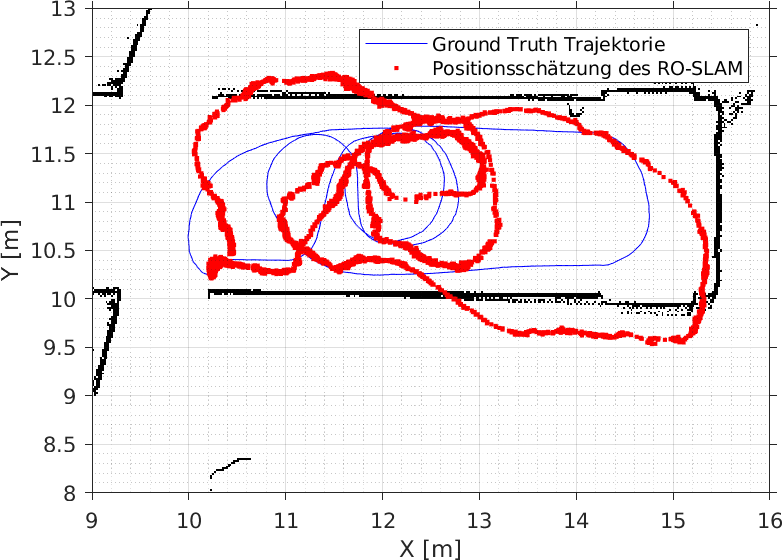
\includegraphics[width=\linewidth]{Record_2018-02-08-12-33-53_filtered_3_trajectory_pf}
			%\caption{Reale UWB Module}
		\end{subfigure}
		\hfill
		\begin{subfigure}{0.41\linewidth}
			\centering
			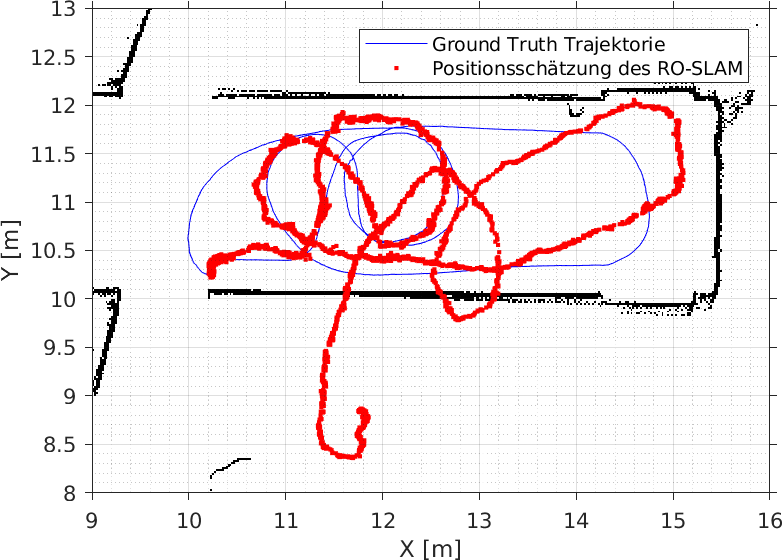
\includegraphics[width=\linewidth]{Record_2018-02-08-12-33-53_filtered_1_trajectory_pf}
			%\caption{Reale UWB Module}
		\end{subfigure}
		\par
		\bigskip
		\begin{subfigure}{0.41\linewidth}
			\centering
			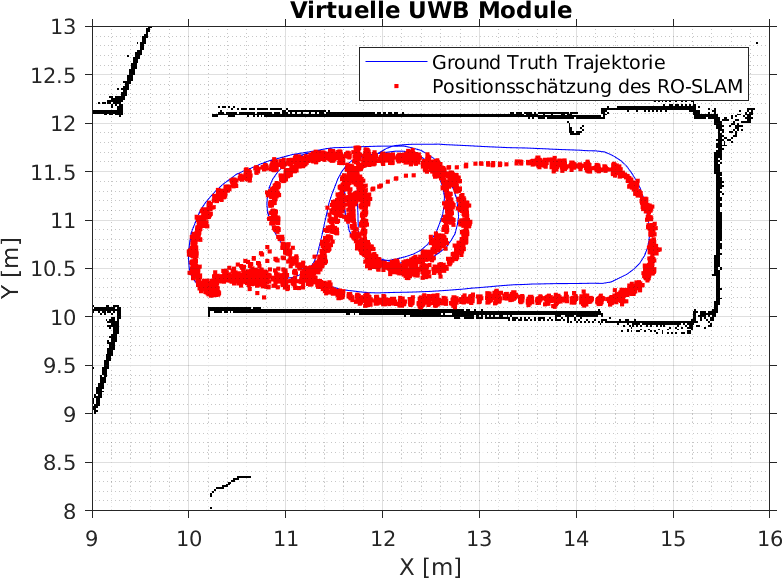
\includegraphics[width=\linewidth]{Record_2018-02-08-12-33-53_filtered_5_trajectory_pf}
			%\caption{Virtuelle UWB Module.}
		\end{subfigure}
		\hfill
		\begin{subfigure}{0.41\linewidth}
			\centering
			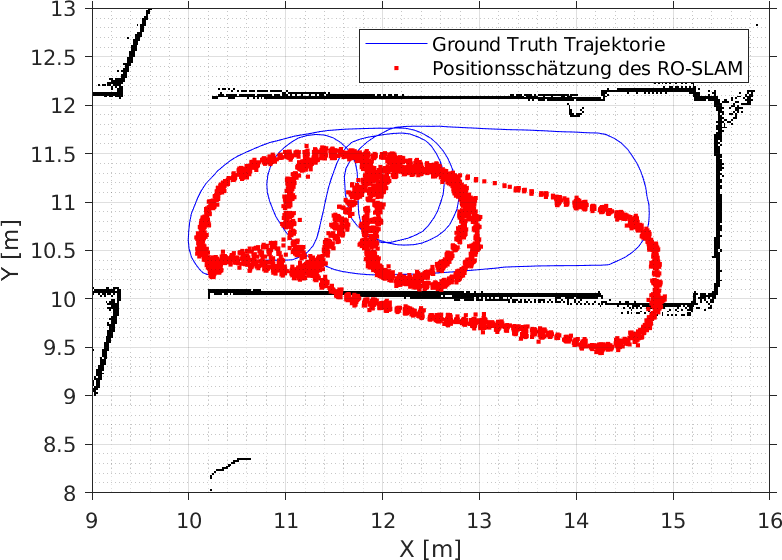
\includegraphics[width=\linewidth]{Record_2018-02-08-12-33-53_filtered_4_trajectory_pf}
			%\caption{Virtuelle UWB Module.}
		\end{subfigure}
	\end{figure}
	
\end{frame}


%%%%%%%%%%%%%%%%%%%%%%%%%%%%%%%%%%%%%%%%%%%%%%%%%%%%%%%%%%%%%%%%%%%%%%%%%%%%%%%%
%
%	- /.../bachelor-thesis/auswertungen/ro_slam_data/viz_bor_mean_cov.m
%
%%%%%%%%%%
\begin{frame}{Positionsschätzung der UWB Module}

	\begin{figure}
		\centering
		\begin{subfigure}{0.41\linewidth}
			\centering
			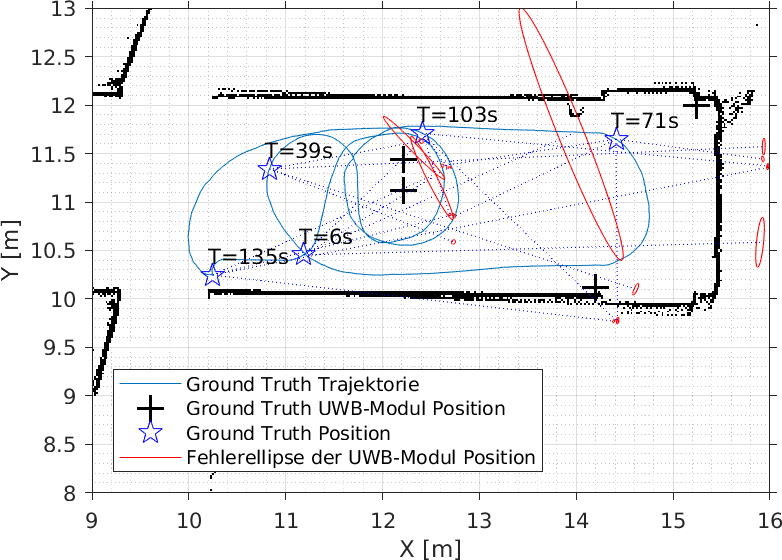
\includegraphics[width=\linewidth]{Record_2018-02-08-12-33-53_filtered_3_beacon_error}
			%\caption{Reale UWB Module}
		\end{subfigure}
		\hfill
		\begin{subfigure}{0.41\linewidth}
			\centering
			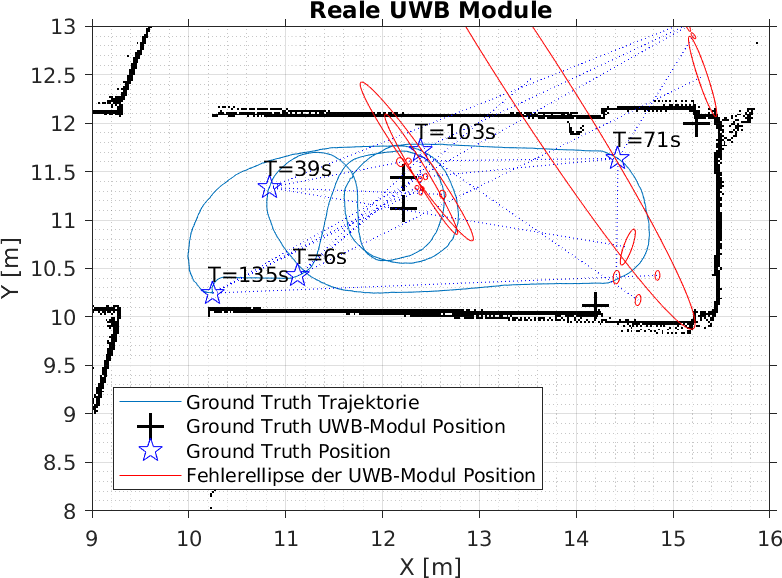
\includegraphics[width=\linewidth]{Record_2018-02-08-12-33-53_filtered_1_beacon_error}
			%\caption{Reale UWB Module}
		\end{subfigure}
		\par
		\bigskip
		\begin{subfigure}{0.41\linewidth}
			\centering
			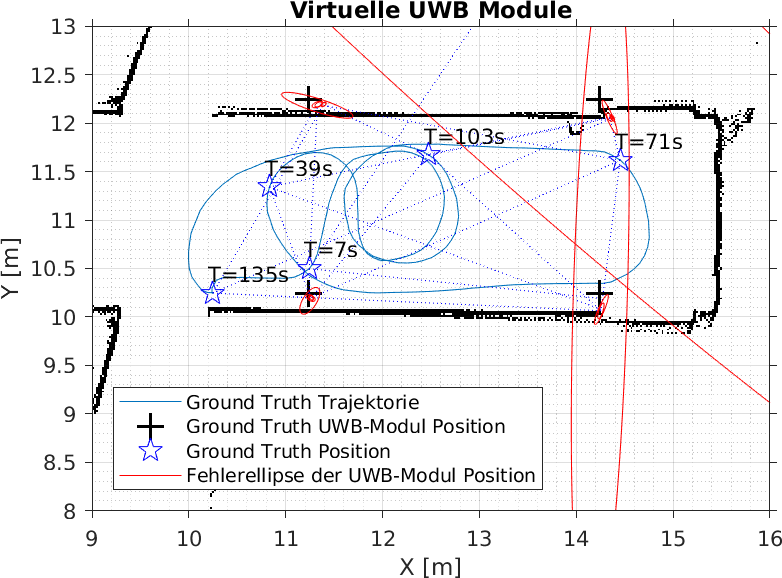
\includegraphics[width=\linewidth]{Record_2018-02-08-12-33-53_filtered_5_beacon_error}
			%\caption{Virtuelle UWB Module}
		\end{subfigure}
		\hfill
		\begin{subfigure}{0.41\linewidth}
			\centering
			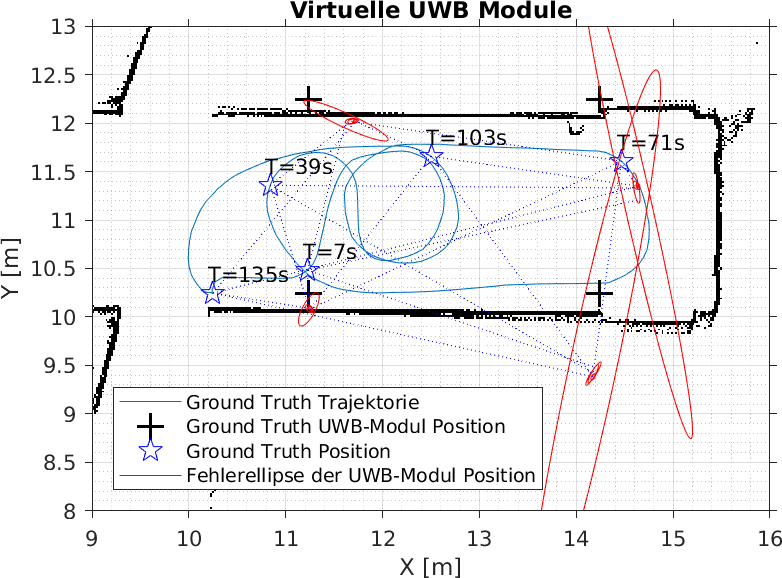
\includegraphics[width=\linewidth]{Record_2018-02-08-12-33-53_filtered_4_beacon_error}
			%\caption{Virtuelle UWB Module}
		\end{subfigure}
	\end{figure}

\end{frame}


%%%%%%%%%%%%%%%%%%%%%%%%%%%%%%%%%%%%%%%%%%%%%%%%%%%%%%%%%%%%%%%%%%%%%%%%%%%%%%%%
%
%	- Beaconfehler durch den Roboter (2018-02-08-13-09-17)
%
%%%%%%%%%%
\begin{frame}
	\frametitle{Fazit}
	\begin{itemize}
		\item UWB Modul
			\begin{itemize}
				\item ...
				\item ...
			\end{itemize}
		\item RO-SLAM
			\begin{itemize}
				\item ...
				\item ...
			\end{itemize}
	\end{itemize}
\end{frame}


%%%%%%%%%%%%%%%%%%%%%%%%%%%%%%%%%%%%%%%%%%%%%%%%%%%%%%%%%%%%%%%%%%%%%%%%%%%%%%%%
%
% 
%
%%%%%%%%%%
\begin{frame}[allowframebreaks]{Literaturverzeichnis}
	\printbibliography[
		heading=bibintoc,
		title={Literaturverzeichnis},
	]
\end{frame}


%%%%%%%%%%%%%%%%%%%%%%%%%%%%%%%%%%%%%%%%%%%%%%%%%%%%%%%%%%%%%%%%%%%%%%%%%%%%%%%%
%
% 
%
%%%%%%%%%%
%\begin{frame}
%\frametitle{Frame Template}
%This is a text in first frame. This is a text in first frame. This is a text in first frame.
%\end{frame}


\end{document}

